%%%%%%%%%%%%%%%%%%%%%%%%%%%%%%%%%%%%%%%%%%%%%%%%%%%%%%%%%%%%%%%%%%%%%%%%%%%%%%%
% This template is distributed with ABSOLUTELY NO WARRANTY.
% It serves as a guideline and constitutes a basic structure for a
% thesis/dissertation. The user assumes full responsibility for formatting
% and typesetting their document and for verifying that all the thesis
% requirements set by the University of Tennessee are met. Please refer to the most
% recent UT thesis guide (http://web.utk.edu/~thesis/thesisresources.shtml)
% or contact the thesis consultant (http://web.utk.edu/~thesis/).
% Please report any bugs to the thesis consultant.
%%%%%%%%%%%%%%%%%%%%%%%%%%%%%%%%%%%%%%%%%%%%%%%%%%%%%%%%%%%%%%%%%%%%%%%%%%%%%%%
% O P T I O N S:
% 1. thesis/dissertation
% 2. monochrome
% 3. all options provided by the report class
\documentclass[thesis,letterpaper,12pt]{utthesis} % thesis, one side
%%%%%%%%%%%%%%%%%%%%%%%%%%%%%%%%%%%%%%%%%%%%%%%%%%%%%%%%%%%%%%%%%%%%%%%%%%%
%                                                                         %
%                                 PREAMBLE                                %
%                                                                         %
%%%%%%%%%%%%%%%%%%%%%%%%%%%%%%%%%%%%%%%%%%%%%%%%%%%%%%%%%%%%%%%%%%%%%%%%%%%

%% LANGUAGE and ENDCODING
\usepackage[english]{babel}
\usepackage{lipsum}
\usepackage[utf8]{inputenc}
\usepackage[T1]{fontenc}

%% PACKAGES
\usepackage[section]{placeins}
\usepackage[usenames,dvipsnames]{xcolor}
\usepackage{microtype}
\usepackage[obeyDraft]{todonotes}
\usepackage{fancyvrb}
\VerbatimFootnotes
\usepackage{algorithmic}
\usepackage{booktabs}
\usepackage{tabularx}
\usepackage{multirow}
\usepackage{longtable}

%% GRAPHICS RELATED
\usepackage{graphicx}
\usepackage[outdir=./tmp/]{epstopdf}
\DeclareGraphicsExtensions{.eps, .pdf, .jpeg, .png}

%% ALGORTHIM
\usepackage[chapter]{algorithm}
\usepackage{algorithmic}

%% CPATION SETUP
\usepackage{float}
\usepackage{caption}
\usepackage{subcaption}
\captionsetup{belowskip=12pt,aboveskip=4pt}

%% UNITS,  EQUATIONS, and CHEMISTRY
\usepackage{textcomp}
\usepackage{siunitx}
\usepackage[version=3]{mhchem}
\usepackage{mathrsfs}

%% NOMENCLATURE
\usepackage[refpage]{nomencl}  % refer to the page where notation appears
\newcommand{\definevar}[2]{#1 is the #2\nomenclature{#1}{#2}}
\newcommand{\nom}[2]{#1 #2\nomenclature{#1}{#2}}
\renewcommand{\nomname}{List of Notations}
\renewcommand*{\pagedeclaration}[1]{\unskip\dotfill\hyperpage{#1}}
\makenomenclature
%%%%%%%%%%%%%%%%%%%%%%%%%%%%%%%%%%%%%%%%%%%%%%%%%%%%%%%%%%%%%%%%%%%%%%%%%%%
%                                                                         %
%                             Listing Setup                               %
%                                                                         %
%%%%%%%%%%%%%%%%%%%%%%%%%%%%%%%%%%%%%%%%%%%%%%%%%%%%%%%%%%%%%%%%%%%%%%%%%%%
\usepackage{listings}
\lstset{ %
    language=C++,
    basicstyle=\footnotesize\ttfamily,
    numbers=left,
    numberstyle=\tiny\color{gray},
    stepnumber=2,
    numbersep=5pt,
    backgroundcolor=\color{white},
    showspaces=false,
    showstringspaces=false,
    showtabs=false,
    frame=single,
    rulecolor=\color{black},
    tabsize=2,
    breaklines=true,
    breakatwhitespace=false,
    title=\lstname,
    keywordstyle=\color{blue},
    commentstyle=\color{OliveGreen},
    stringstyle=\color{orange}
}
\DeclareCaptionFont{white}{\color{white}}
\DeclareCaptionFormat{listing}{\colorbox[cmyk]{0.43, 0.35, 0.35, 0.01}{\parbox{\dimexpr\textwidth-2\fboxsep\relax}{#1#2#3}}}
\captionsetup[lstlisting]{format=listing,labelfont=white,textfont=white,singlelinecheck=false,margin=0pt,font={bf,footnotesize}}

%% USER COMMANDS
\usepackage{isotope}
\newcommand{\iso}{\isotope}
\newcommand{\figurewidth}{\textwidth}
\DeclareSIUnit\roetgen{R}
\DeclareSIUnit\eV{\electronVolt}
\DeclareSIUnit\count{count}
\DeclareSIUnit\rem{rem}
\DeclareSIUnit\in{in}
\DeclareSIUnit\cps{\count\per\second}
\DeclareSIUnit\cpsngcf{\count\per\second\per\nano\gram\iso[252]{Cf}}

%% Table of Contents
\addto\captionsenglish{%
 \renewcommand{\contentsname}{Table of Contents}%
}

\usepackage{termcal}
\usepackage{pgfgantt}
\usepackage{rotating}
\usepackage{tikz}
\usetikzlibrary{shapes,arrows}
\usepackage{dot2texi}
% some alternatives are:
%\documentclass[thesis,monochrome,letterpaper,12pt]{utthesis} %thesis, one side, monochrome text
%\documentclass[thesis,twoside,letterpaper,12pt]{utthesis} % thesis, two side
%\documentclass[thesis,monochrome,twoside,letterpaper,12pt]{utthesis} % thesis, two side, monochrome text
% for a dissertation, replace the thesis option by dissertation:
% \documentclass[dissertation,letterpaper,12pt]{utthesis} . . .
\renewcommand{\baselinestretch}{1.5} 	 % line Spacing
%%%%%%%%%%%%%%%%%%%%%%%%%%%%%%%%%%%%%%%%%%%%%%%%%%%%%%%%%%%%%%%%%%%%%%%%%%%%%%%
% TO DO: FILL IN YOUR INFORMATION BELOW - READ THIS SECTION CAREFULLY
%%%%%%%%%%%%%%%%%%%%%%%%%%%%%%%%%%%%%%%%%%%%%%%%%%%%%%%%%%%%%%%%%%%%%%%%%%%%%%%
\title{Optimization of the Radiation Portal Monitor}
\author{Matthew J. Urffer}
\date{August 9, 2013}
\copyrightYear{2013} 
\graduationMonth{December}
\majorProfessor{Liaurence F. Miller}
\keywords{Neutron Detectors, Radiation Portal Monitors, GEANT4, MCNPX, Simulation}
\college{Engineering}
\dept{Nuclear Engineering}
\university{The University  of Tennessee, Knoxville}
\viceProvost{Carolyn R. Hodges}
\major{Nuclear Engineering}
\degree{Doctor of Philosophy}
\college{Engineering}
\dept{Nuclear Engineering}
\university{The University  of Tennessee, Knoxville}
\numberOfCommitteeMembers{3}
\committeeMemberA {Lawrence H. Heilbronn}
\committeeMemberB {Dayaker Penumadu}
\committeeMemberC {Ronald E. Pevey}
%%%%%%%%%%%%%%%%%%%%%%%%%%%%%%%%%%%%%%%%%%%%%%%%%%%%%%%%%%%%%%%%%%%%%%%%%%%%%%%
% LOAD SOME USEFUL PACKAGES
%%%%%%%%%%%%%%%%%%%%%%%%%%%%%%%%%%%%%%%%%%%%%%%%%%%%%%%%%%%%%%%%%%%%%%%%%%%%%%%
\graphicspath{{tmp/}{figures/}{figures/eps/}{figures/pdf/} }% specify the path where figures are located
\usepackage{fancyhdr}                   % fancy headers and footers
\usepackage[inactive]{srcltx}		 	% necessary to use forward and inverse searching in DVI
\usepackage{relsize}                    % font sizing hierarchy
%%%%%%%%%%%%%%%%%%%%%%%%%%%%%%%%%%%%%%%%%%%%%%%%%%%%%%%%%%%%%%%%%%%%%%%%%%%%%%%
\begin{document}
    \pagenumbering{alph} % this is needed to clear certain issues with the hyperref package
    %
    %
    \addToPDFBookmarks{0}{Front Matter}{rootNode} % create a root node named "Front Matter" in the pdf bookmarks
    \addToPDFBookmarks{1}{Title}{a} % add a pdf bookmark to the title page
    \maketitle
    %
    \pagenumbering{roman}
    \setcounter{page}{2}
    %
    \addToPDFBookmarks{1}{Dedication}{b} % add a pdf bookmark to the dedication page
    \chapter*{}
\begin{center}
{\centering \textit{To my family and friends}}
\vspace{2 cm}
\begin{figure}[h]
\centering

\includegraphics[width=0.5\textwidth]{tryScience}
\end{figure}
\end{center} 

 % include the dedication
    %
    \addToPDFBookmarks{1}{Acknowledgements}{c} % add a pdf bookmark to the acknowledgements page
    \chapter*{Acknowledgments}

This works would not have been possible without the support of many different people.
Dr. Miller has been an essential resource for bouncing ideas around while providing valuable insights and supporting this work.
I would also like to thank my committee members, Dr. Heilbronn, Dr. Penumadu, and Dr. Pevey, for their support and technical expertise that they have provided. 
The testing of films would not have been possible without the kind folks fabricating the materials, I would like to acknowledge the work of Dr. Mabe, Dr. Auxier II, and Dr. Uppal for their help and numerous conversations.

The academic portion of this would would have never succeeded without the support from my friends and family. 
My mother and father, Lisa and Micheal, deserve special recognition of their support, encouragement and frank advice. 
Katie, Samuel, David, Isaac, Esther and Eli also deserve recognition for their support and efforts. 
Finally, I would like to thank the members of Knoxville Ultimate for being supportive and offering many great games.
 % include the acknowledgements
    \addToPDFBookmarks{1}{Abstract}{d} % add a pdf bookmark to the title page
    \begin{abstract}
    \chapter*{Abstract}
\label{chap:abstract}
Alternative neutron detection technologies are required to replace the current He-3 based Radiation Portal Monitors (RPM) which are employed to detect special nuclear material that may be entering the United States illicitly.
Replacement technologies must fulfill the following criteria established by the Department of Homeland Security: 1) a neutron detection efficiency, 2) a gamma insensitivity, and 3) the performance of the detector should not suffer in the the presence of a strong gamma field.
Polymeric films containing Li-6 ranging from 15 to 300 microns have the ability to fulfill these criteria if suitably utilized.
For a typical detector material the design involves maximizing the neutron-gamma discrimination, maximizing the physical detector configuration in order to ensure optimal use of the incident neutron spectra, and ensuring that the scintillation light generated can be collected.

A technique for using a pulse height discriminator for rejecting gamma interactions has been determined for polymeric films  ranging from 15 microns to 300 microns in thickness.
The basis of this technique has been attributed to the relative ranges of the secondary electrons of the Compton scattered electrons (generally in the hundred of keV) from the gamma interactions, compared to the ranges of the electrons from the reaction products of a neutron absorption, which have energies int he 10 keV range.
Detailed Monte Carlo simulations indicate that a desired film thickness is around 100 microns.

A replacement portal monitor has been designed for layered polymeric films that effectively utilize enriched Li-6 in the detector material using a genetic algorithm to optimize the spacing between the layers, while cylindrical designs could also be employed.
If two photomultiplier tubes are placed at the top and bottom of a fishtail light guide mounted on the top and bottom of the detector cabinet, eight precent of the optical photons generated in a 10 precent loaded polystyrene film can be collected, leaving an acceptable number of photons to create a signal.

    \end{abstract}
    %
    \pagenumbering{roman}
    \setcounter{page}{2}
    %
    \addToPDFBookmarks{1}{Table of Contents}{e}
    \tableofcontents % generate a table of contents
    %
    \addToPDFBookmarks{1}{List of Tables}{f}
    \listoftables % generate a list of tables
    %
    \addToPDFBookmarks{1}{List of Figures}{g}
    \listoffigures % generate a list of figures
    %
    \makenomenclature % OPTIONAL
    \addToPDFBookmarks{1}{Nomenclature}{h} % OPTIONAL
    \printnomenclature[1.25in] % OPTIONAL
    %
    \newpage
    \pagenumbering{arabic}
    \setcounter{page}{1}
    %%%%%%%%%%%%%%%%%%%%%%%%%%%%%%%%%%%%%%%%%%%%%%%%%%%%%%%%%%%%%%%%%%%%%%%%%%%
    % INCLUDE THE CHAPTERS STARTING WITH THE NOMENCLATURE IF PRESENT
    %%%%%%%%%%%%%%%%%%%%%%%%%%%%%%%%%%%%%%%%%%%%%%%%%%%%%%%%%%%%%%%%%%%%%%%%%%%
    %%%%%%%%%%%%%%%%%%%%%%%%%%%%%%%%%%%%%%%%%%%%%%%%%%%%%%%%%%%%%%%%%%%%%%%%%                                                                        %
%                         PROJECT INTRODUCTION                            %
%                                                                         %
%%%%%%%%%%%%%%%%%%%%%%%%%%%%%%%%%%%%%%%%%%%%%%%%%%%%%%%%%%%%%%%%%%%%%%%%%%%
\chapter{Introduction} 
\label{ch:Intro}
Radiation Portal Monitors (RPMs) are passive radiation detection systems implemented at over a thousand of border crossings, designed to determine if cargo contains any special nuclear material in a safe, nondestructive, and effective manner\cite{kouzes_neutron_2010}. 
However, the current technology used in RPMs for detecting neutrons emitted from special nuclear material use a rapidly diminishing resource, \iso[3]{He}, that cannot be economically replaced. 
The Department of Homeland Security (DHS) continues to fund research (through the Domestic Nuclear Detection Office (DNDO)) for the development of detector systems to detect radioactive material that could potentially be used to cause significant economic loss and loss of life.  
As a result of this research a number of alternative detection systems continue to be investigated with the most viable including: boron trifluoride filled proportional detectors, boron-lined proportional detectors, \iso[6]{Li} loaded scintillation glass fiber detectors, and \iso[6]{Li} plus scintillator-coated wavelength-shifting fiber detectors\cite{pnnl_18471,kouzes_neutron_2010}.  

Neutron detectors often utilize a material with a large cross section for absorption, such as \iso[6]{Li} or \iso[10]{B}.
When these materials absorb a neutron they usually disintegrate to produce ionized reaction products that in turn transfer their kinetic energy to electrons.
In the case of the $\iso[6]{Li}\left(n,\iso[3]{H}\right)\alpha$ reaction, the fission energy is distributed between a triton of energy \SI{2.73}{\mega\eV} and an alpha of energy \SI{2.05}{\mega\eV}.
In a proportional counter such as the \iso[3]{He} based detectors,the energy from the charged particles would ionize a gas, creating a voltage signal.
Scintillator detectors, on which this work is based, utilize the charged particle energy depositions to create electron excitations in the scintillating material which are then harvested by fluors and produce visible light, which is detected with a photomultiplier tube.


\section{Replacement Detector Criteria}
\label{sec:ReplacmentCriteria}
Pacific Northwest National Lab (PNNL) along with the DNDO have developed a set of specifications that that replacement RPMs must meet \cite{kouzes_neutron_2010, kouzes_neutron_1999}. 
In particular 1) an absolute neutron detection efficiency greater than \SI{2.5}{\cps} at \SI{2}{\meter} for a defined moderated  source, 2) an intrinsic gamma-neutron detection efficiency of one in a million, and 3) a gamma absolute rejection ratio for neutrons stating that the performance of the detector should not change by more than 10\% in a \SI{10}{\milli\roetgen\per\hour} gamma field.
These parameters are summarized in \autoref{tab:DHSCritera}.
\begin{table}
  \centering
	\caption{Replacement Portal Monitor Criteria}
	\begin{tabular}{m{8cm} m{6cm} }
	Parameter & Specification \\
	\hline
	\hline
	Absolute neutron detection efficiency & 2.5 cps/ng of \iso[252]{Cf} (in specified test configuration) \\
	Intrinsic gamma-neutron detection efficiency & $ \epsilon_{int,\gamma n}\leq 10^{-6}$ \\
	Gamma absolute rejection ratio for neutrons (GARRn) & $ 0.9 \leq \text{ GARRn }\leq$ 1.1 at 10 mR/h exposure \\
	Cost &  \$ 30,000 per system \\
	\end{tabular}
	\label{tab:DHSCritera}
\end{table}

The absolute neutron detection efficiency $\left (\epsilon_{abs,n} \right )$ is defined as the number of neutron pulses recorded by the detector normalized by the number of neutrons emitted by the source as shown in \autoref{eqn:absn}
\begin{align}
	\label{eqn:absn}
  \epsilon_{abs,n} = \frac{N_{nc}}{N_{ns}}
\end{align}
where \definevar{$N_{nc}$}{neutron count rate} and \definevar{$N_{ns}$}{neutron emission rate from the source}.
DNDO guidelines state that a \iso[252]{Cf} source placed \SI{2}{\meter} from the midpoint of the detector is to be used for the determination of the absolute neutron detection efficiency\cite{pnnl_18471}.
To reduce the gamma ray flux of \iso[252]{Cf} upon a candidate detector the source is shielded by at least \SI{0.5}{\cm} of lead, and the neutron spectrum is then moderated by \SI{2.5}{\cm} of polyethylene\cite{pnnl_18471}.
The intrinsic efficiency, which provides a measure of how sensitive the detector is to incoming radiation, is defined in \eqref{eqn:inteff}.
\begin{align}
  \label{eqn:inteff}
  \epsilon_{int} = \frac{\text{Number Counts Observed}}{\text{Number Quanta for Radiation Crossing Detector}}
\end{align}
The formulation presented in \eqref{eqn:inteff} is then adapted to photons, with the requirement that only one count per a million photons passing through the detector may be registered.
To account for this the subscript $\gamma n$ is added to the intrinsic efficiency \eqref{eqn:inteffNG}
\begin{align}
  \label{eqn:inteffNG}
  \epsilon_{int,\gamma n} &= \frac{P_{pc}}{P_{p\Phi}}
\end{align}
where \definevar{$P_{pc}$}{photon count rate} and \definevar{$P_{p\Phi}$}{photons crossing the detector}.
The intrinsic gamma-neutron detection efficiency is to be measured using either a \iso[192]{Ir}, \iso[137]{Cs}, or \iso[60]{Co} source placed at an appropriate distance so as to produce an exposure rate of \SI{10}{\milli\roetgen\per\hour} at the detector\cite{kouzes_neutron_1999}.
The final detector parameter, the gamma absolute rejection ratio (GARRn), characterizes the detector response in the presence of both a large gamma ray source (\SI{10}{\milli\roetgen\per\hour}) and a \iso[252]{Cf} neutron source (configured as it would be for an absolute neutron detection efficiency measurement).
This criteria, shown in \eqref{eqn:garrn}, implies that the performance of the detector should not change by more than 10\% in a strong gamma field\cite{kouzes_neutron_1999}.
\begin{align}
  \label{eqn:garrn}
  GARRn = \frac{ \epsilon_{abs,\gamma n}}{\epsilon_{abs,n}}
\end{align}

%%%%%%%%%%%%%%%%%%%%%%%%%%%%%%%%%%%%%%%%%%%%%%%%%%%%%%%%%%%%%%%%%%%%%%%%%%%
%                                                                         %
%                       CURRENT TECHNOLOGIES                              %
%                                                                         %
%%%%%%%%%%%%%%%%%%%%%%%%%%%%%%%%%%%%%%%%%%%%%%%%%%%%%%%%%%%%%%%%%%%%%%%%%%%
\section{Current Technologies}
\label{sec:CurrentTechnologies}
Currently a number of alternative technologies are being developed, but two of the most promising detector technologies are boron loaded straw fibers being developed by Proportional Technologies Inc. (Houston, TX) and LiF loaded ZnS(Ag) scintillator paddles being developed by Innovative American Technology (Coconut Creek, FL).
The boron straw tubes meet the count rate criteria with a gamma rejection rate estimated at \num{4e-9} while passing the GARRn \cite{kouzes_boron-lined_2012}.
LiF/ZnS(Ag) is a commercial inorganic scintillator utilizes the alpha from the \iso[6]{Li} neutron capture to active the ZnS doped with silver (ZnS(Ag)). 
LiF/ZnS(Ag) has a high light output per neutron (\num{1.6E5} photons per neutron) with a decay time of approximately \SI{100}{\micro\second} and the maximum emission at \SI{450}{\nm} \cite{carel_w.e_inorganic-scintillator_2001}.
However, this material is opaque and therefore care needs to be taken with the light collection of a large area detector.
Innovative American Technology (IAT) has developed a design of a replacement RPM that utilizes LiF/ZnS(Ag), as shown schematically in \autoref{fig:IATRender} and in \autoref{fig:IATImage}.
Current testing indicates that this detector design will meet the DHS criteria\cite{kouzes_lithium_2010}.
\begin{figure}
  \centering
  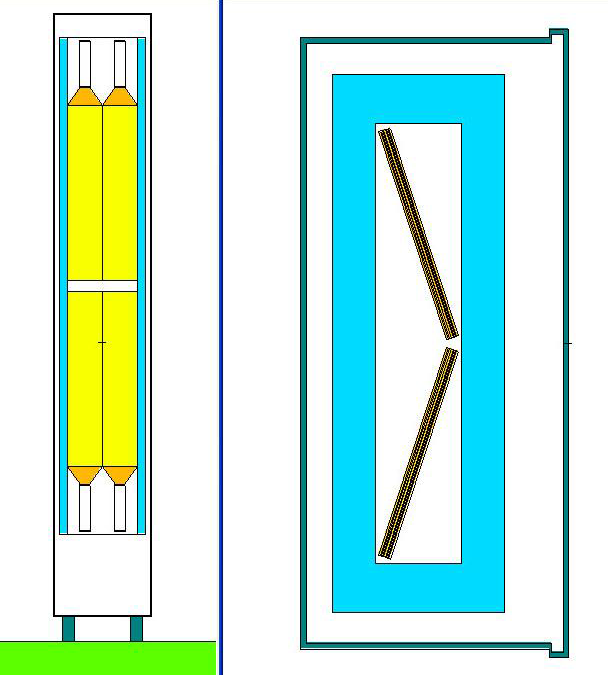
\includegraphics[width=0.5\textwidth]{IATRender}
	\caption[Rendering of IAT Neutron Detector]{Modeled IAT detector that consist of four paddles.  The paddles are angled to expose a larger surface to the neutron flux\cite{pnnl_22228}.}
	\label{fig:IATRender}
\end{figure}
\begin{figure}
  \centering
  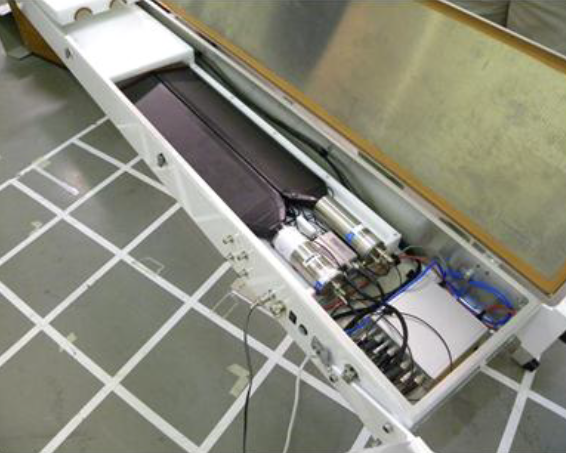
\includegraphics[width=0.75\textwidth]{IATImage}
	\caption[Photograph of IAT Neutron Detector]{Photograph of the developed IAT detector\cite{pnnl_22228}.}
	\label{fig:IATImage}
\end{figure}

%%%%%%%%%%%%%%%%%%%%%%%%%%%%%%%%%%%%%%%%%%%%%%%%%%%%%%%%%%%%%%%%%%%%%%%%%%%
%                                                                         %
%                       DEVELOPED SCINTILLATORS                           %
%                                                                         %
%%%%%%%%%%%%%%%%%%%%%%%%%%%%%%%%%%%%%%%%%%%%%%%%%%%%%%%%%%%%%%%%%%%%%%%%%%%
\section{Developed Scintillators}
\label{sec:DevelopedScintillators}
In addition to the inorganic scintillator LiF/ZnS(Ag), work is being completed at the University of Tennessee to construct thin film polymeric scintillators to be utilized in a layered detector design for replacement RPMs.
These films, either based on polystyrene (PS) or polyethylene naphthalate (PEN), are \iso[6]{LiF} containing polymers projected to be low cost, have high mechanical durability, and meet the detector criteria \cite{Sen_Composites,Mabe201329}.
The developed materials have been characterized for their neutron performance and gamma discrimination abilities, a summary of which (as of May 2013) may be found in \autoref{ch:MeasuredFilmPerfomance}.
%%%%%%%%%%%%%%%%%%%%%%%%%%%%%%%%%%%%%%%%%%%%%%%%%%%%%%%%%%%%%%%%%%%%%%%%%%%
%                                                                         %
%                       OPTIMIZATION INTRODUCTION                         %
%                                                                         %
%%%%%%%%%%%%%%%%%%%%%%%%%%%%%%%%%%%%%%%%%%%%%%%%%%%%%%%%%%%%%%%%%%%%%%%%%%%
\section{Optimization Opportunities}
There exists a need to build predictive modeling capabilities of these detectors in order to optimize the detector performance.
For a particular material and neutron absorber the detector geometry can be optimized to maximize the energy deposited in scintillation material by charged particles relative to the energy deposited by photon interactions. 
This in turn permits one to maximize the recorded neutron interaction rate relative to recorded photon interaction rates by setting a lower level discriminator (LLD) above a threshold associated with energy deposited in the detector by photons.  
As the LLD is increased, the efficiency for detecting neutrons is diminished; however, the intrinsic efficiency for detecting neutrons relative to photons is dramatically increased. 
In addition, as the neutron flux is being moderated and absorbed by the RPM material there exist the opportunity to position the neutron absorber films to maximize the neutron count rate while minimizing the amount of material being used.
Finally, it is essential to ensure that the scintillation light can be collected efficiency.

%%%%%%%%%%%%%%%%%%%%%%%%%%%%%%%%%%%%%%%%%%%%%%%%%%%%%%%%%%%%%%%%%%%%%%%%%%%
%                                                                         %
%                       ORGINAL CONTRIBUTION                              %
%                                                                         %
%%%%%%%%%%%%%%%%%%%%%%%%%%%%%%%%%%%%%%%%%%%%%%%%%%%%%%%%%%%%%%%%%%%%%%%%%%%
\section{Original Contribution}
\label{sec:OrginalContribution}
The design of effective radiation portal monitors is a critical component in detecting and subsequent interdiction of special nuclear material.
Most researchers assume that adequate neutron-gamma discrimination can be achieved by the relatively low mass attenuation coefficient for polymers and taking advantage of the thinness of a detector, but for a common plastic based scintillator the detector would have to be less than \SI{160}{\nm} in order to have an interaction rate less than one in a million.
This work is unique in that the fundamental physics basis of the neutron-gamma discrimination is not attributed to the mass attenuation coefficient but rather to the ranges of the secondary electrons from photon interactions in the material depositing less energy than their neutron counterparts.
Current modeling work in large area neutron detectors focuses either with monolithic plastic slab geometries or with neutronic calculations that do account for light collection and transport.
A layered detector design, while not unique, has not been optimized using a genetic algorithm for which the formulation or the problem is quite natural.
In addition, little modeling work has been completed on the performance of a radiation portal monitor including light transport, which is a large majority of this work.
  % Problem introduction
    \chapter{Proposed Work and Methodology}
\label{ch:ProposedWorkAndMethodology}
Advanced modeling of detector designs will allow for the optimization of a radiation portal monitor in order to ensure effective use of the detector materials and the signals they generate while acheiving desirable performance.
The optimization of a radiation portal monitor can be thought as the optimization of the individual components, namely:
\begin{itemize}
  \item the optimization of the neutron and gamma discrimination through the energy deposition,
  \item the optimization of the neutron interaction rates,
  \item the optimization of the detector to minimize scintillation light loss.
\end{itemize}
%The optimization is divided into three components, and as such each of components will be presented individually.
The optimization of the neutron and gamma discrimination will be proposed in \autoref{sec:NGDiscrim} in which high fidelity energy deposition modeling is proposed to study the fundamental interactions leading to the light yield of photon and neutron events.
It is proposed in \autoref{sec:RPMNP} to study the neutronics of layered scintillator RPM detectors designs and then optimize a layered RPM detector design with an advanced search techniques.
Finally, it is proposed to study an entire detector design including the light production, transport, and collection in \autoref{sec:RPMLCP} to ensure a workable and effective detector design.

\section{Neutron - Gamma Discrimination}
\label{sec:NGDiscrim}

Effective neutron-gamma discrimination is integral to the performance of the detector.
Generally, two methods are available for discrimination; 1) pulse shape discrimination and 2) pulse height discrimination.
In pulse shape discrimination the different decay times between the neutron and gamma pulses are exploited to develop a metric that allows for the classification of the pulse.
Generally, pulse shape discrimination works best when the pulses are noticeably different.
Pulse height discrimination is based on setting a pulse height discriminator that acts as a partition between two classes of pulses.
This is generally easier to implement than pulse shape discrimination.
While some of the fabricated films show a small basis for pulse shape discrimination, this work will only focus on pulse height discrimination.

The pulse height discriminator setting necessary to achieve the neutron-gamma discrimination is achieved through the use of a mathematical lower level discriminator (MLLD).
This virtual discriminator establishes the bound where $\epsilon_{int,\gamma n}\leq 10^{-6}$, and counts above the MLLD are classified as neutron counts. 

It is currently understood that the light output per path length of the film (which is directly proportional to the pulses collected on the PMT) is related to the stopping power of the radiation in the film material.
This is described by the Birks equation \eqref{eqn:BirksEquation}
\begin{align}
  \label{eqn:BirksEquation}
  \frac{dL}{dx} = \frac{S_B\frac{dE}{dx}}{1+kB\frac{dE}{dx}}
\end{align}
where \definevar{$S_B$}{absolute scintillation efficiency},\definevar{$\frac{dE}{dx}$}{linear stopping power} and \definevar{$kB$}{Birks parameter}.
For a given material the stopping power of the film will be constant, and therefore the light output of the film can be found by integrating the light output per path length over the total length of the film.
It is then possible to observe that the light output of a film is proportional to the energy deposited in the film.
\subsection{Proposed Work}
It is proposed to optimize the neutron-gamma discrimination by focusing on the energy deposition in the film.
Preferential energy deposition by neutrons relative to gammas will enhance the discrimination by creating larger neutron light pulses than the gamma pulses, allowing for fewer neutron pulses to be classified as gamma pulses because they are below the MLLD.
The product of this work will be a measurement validated simulation capability for the energy deposition in polymeric films (focusing on polystyrene).
The simulation capability will be applied to the optimization of the polystyrene film system.
\subsection{Methodology}

The GEANT4 toolkit has the ability to track the energy deposition in different materials as well as the tracking of electrons to a least \SI{1}{\keV}\cite{agostinelli_geant4simulation_2003}.
It is proposed to represent the detector geometry as a single layer of neutron absorbing thin polymeric film mounted on top of a non-scintillating material (PMMA).
For simplicity, the initial events for runs will be chosen by setting up a particle gun for thermal (\SI{0.025}{\eV}) neutrons upon the detector and for both gammas resulting from a \iso[60]{Co} decay.
\begin{figure}
  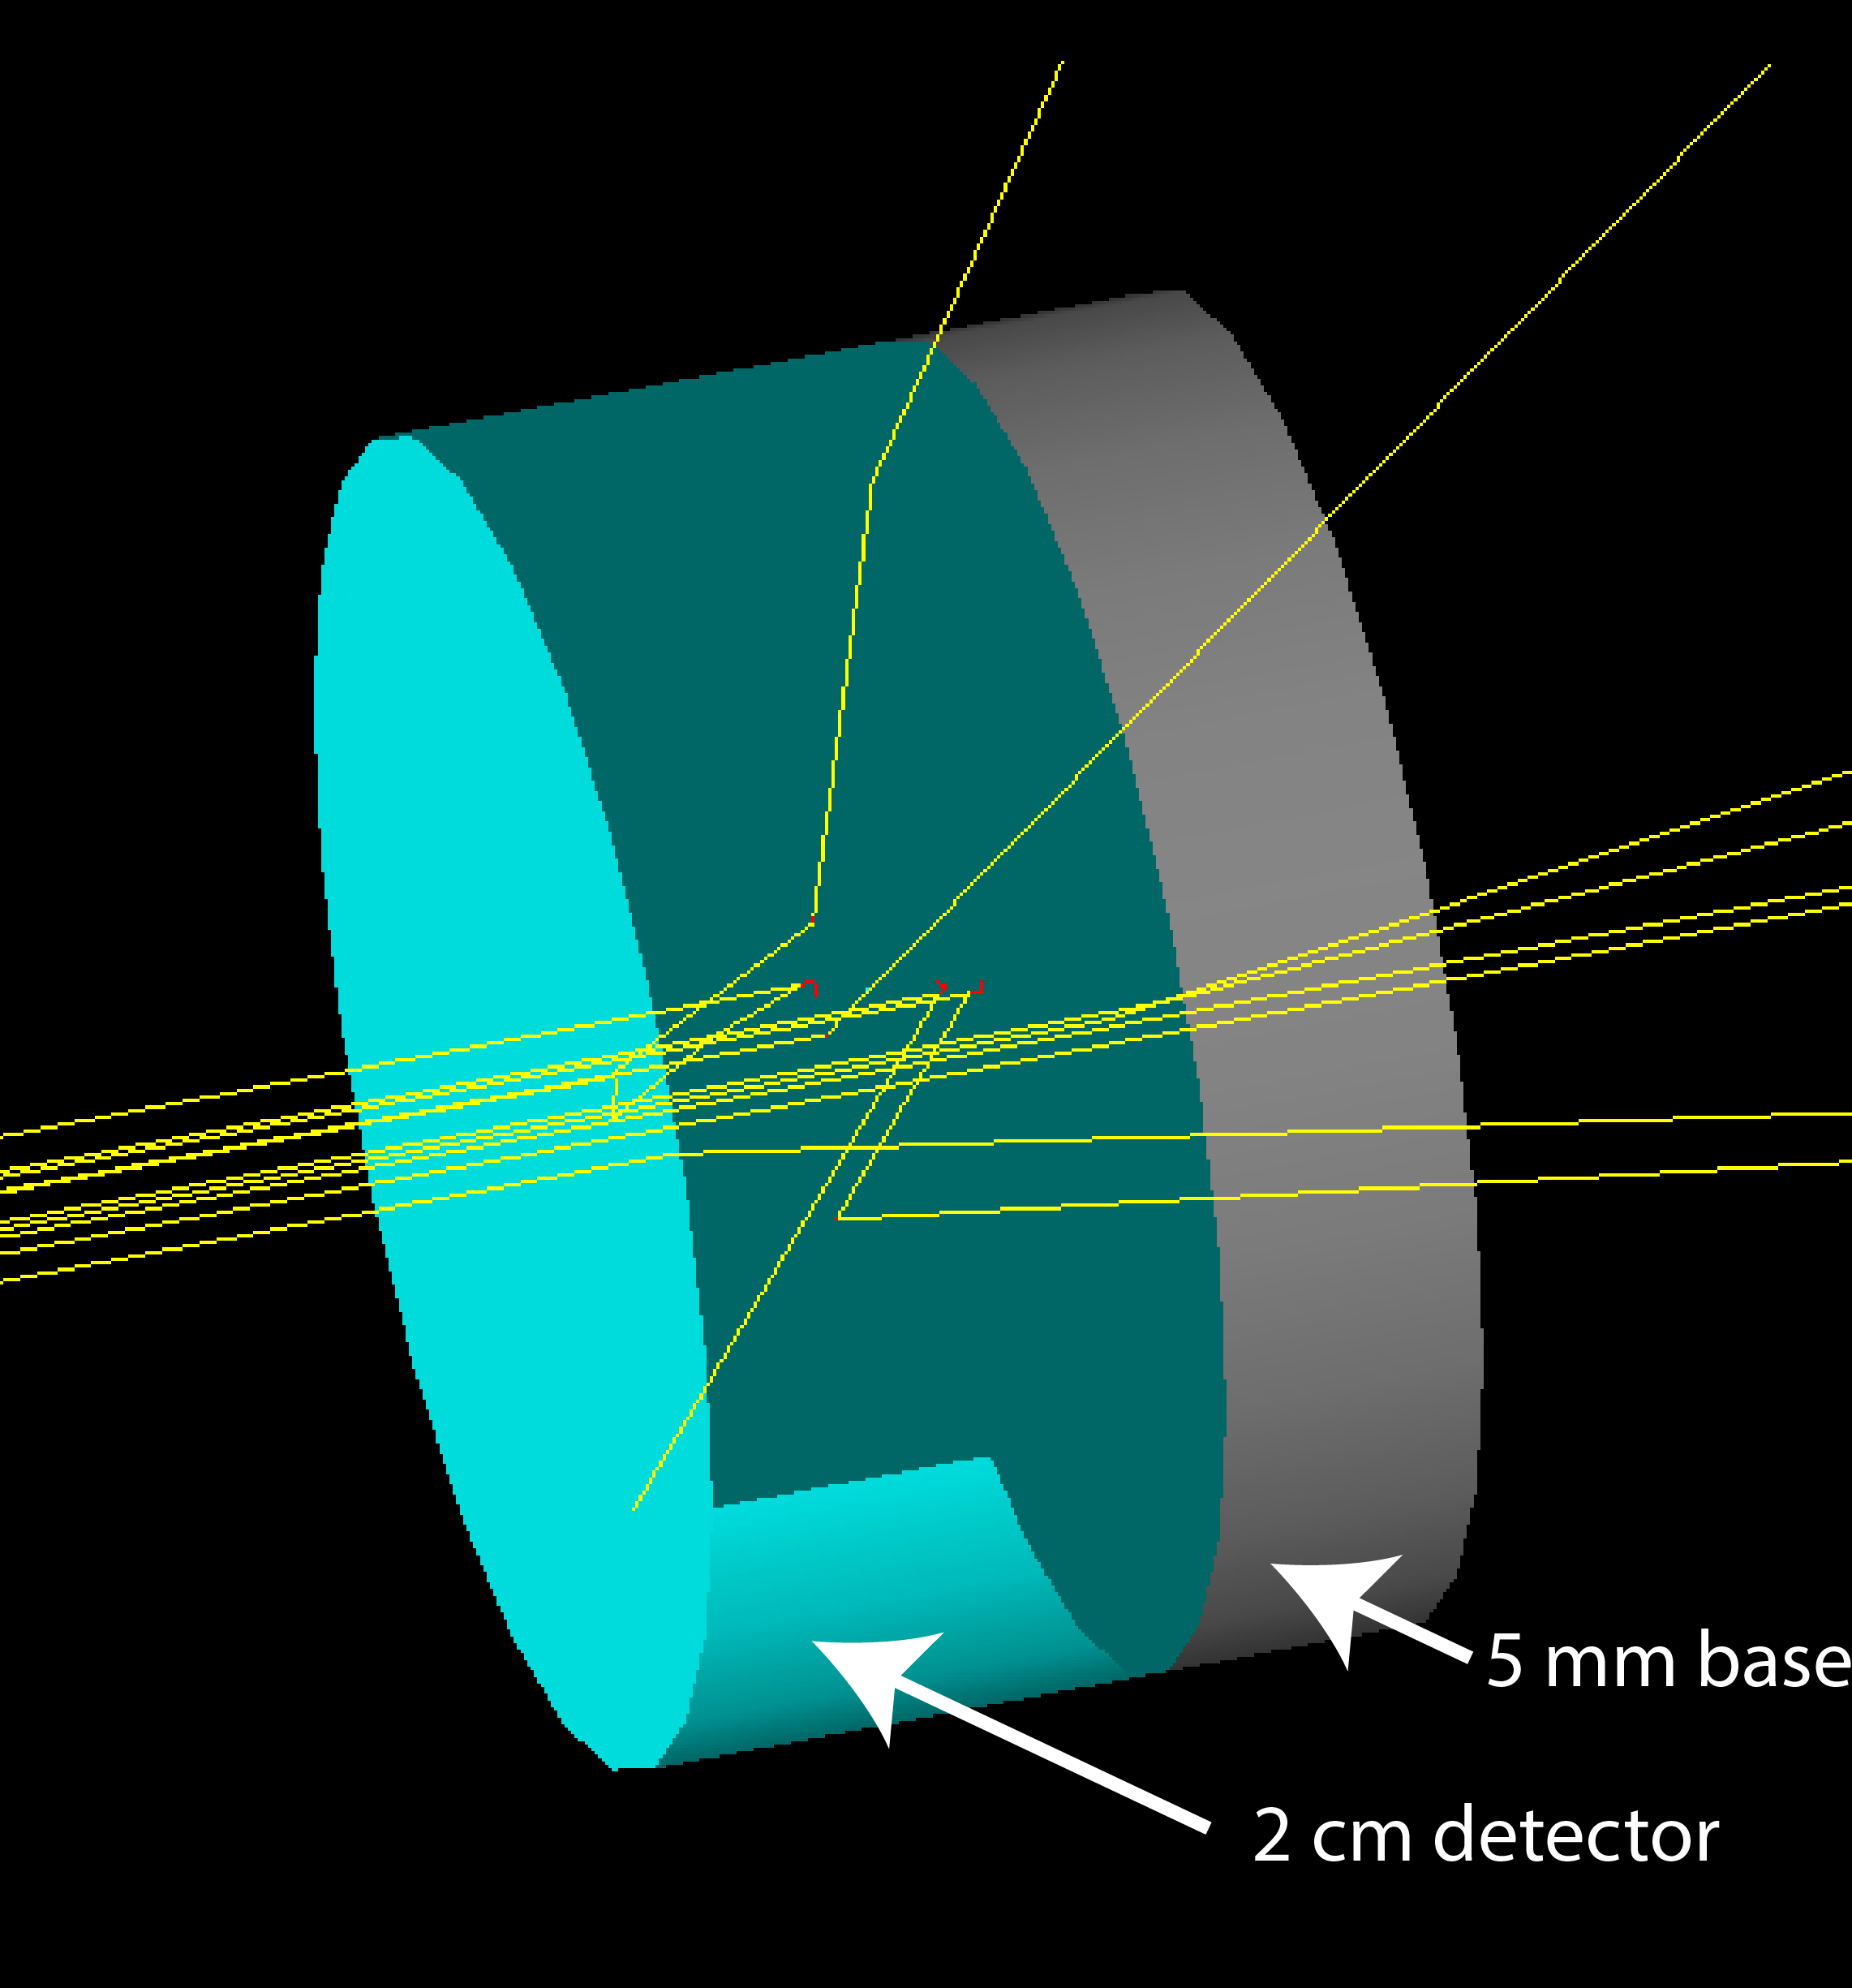
\includegraphics[width=\textwidth]{GEANT4AnnotatedGeo_EnergyDepEvent}
	\caption[GEANT4 Energy Depostion Geometry]{GEANT4 Geometry for the Simulation of Energy Deposition. What is shown are 10 photons from a \iso[60]{Co} source impigent upon a \SI{2}{\cm} thick detector.  The photon tracks are shown in yellow, while the electron tracks are shown in red.}
	\label{fig:EDepSimGeo}
\end{figure}
It is expected that the the Livermore data-driven parameterized electromagnetic physics will be necessary to calculate the ionizing energy deposition, extending the standard electro-magnetic physics down to \SI{1}{\kilo\eV}.
The neutron interactions will be simulated with a hadronic modules, using the \verb+HP+ flavored modules to use the ENDF cross sections to calculate the interaction rates.

It is proposed to validate the simulation by reproducing the single collision energy loss in water as well as comparing  the spectral shapes and averages of simulated and measured spectra.
The reproduction of the single collision energy loss will ensure that the electron physics are implemented correctly, while the simulation of the polymeric film energy deposition allows the user to gain confidence that the correct tracking and binning analysis has been implemented.
%%%%%%%%%%%%%%%%%%%%%%%%%%%%%%%%%%%%%%%%%%%%%%%%%%%%%%%%%%%%%%%%%%%%%%%%%%
%                                                      									 %
%                  		  	RPM Neutronic Performance   		            	 %
% 									                                                     %
%%%%%%%%%%%%%%%%%%%%%%%%%%%%%%%%%%%%%%%%%%%%%%%%%%%%%%%%%%%%%%%%%%%%%%%%%%
\section{RPM Neutronic Performance}
\label{sec:RPMNP}

Simulations are necessary to guide the design of a replacement RPM.
These simulations must provide a link between the measured performance of laboratory developed and characterized samples which are generally two inches and the performance of the film in an implemented detector system as it is prohibitive to construct and measure each film in an RPM.
Previous work showed that it is possible to adequately simulate detector performance in MCNPX, a Monte Carlo radiation transport code.
Generally these simulations involve correctly defining the simulation physics, source and geometry, and then using the correct tally measures to extract pertinent performance metrics.
After the simulation is completed is then benchmarked against measured quantities to provide a measure of confidence that the simulation provides an accurate model of reality.
Often (as in this case) the capability to directly measure the performance of the desired simulation geometry is not availabl is not available, and therefore the benchmarking must be completed on a comparable system on which it is possible to measure.

A validated simulation capability allows for one to explore the design space without having to physically build and test systems, which can be prohibitively expensive.
As a single film does not have the necessary interactions to fulfill the neutron count rate criteria multiple films are necessary, and the arrangement of these films provides a design space for a replacement RPM.
In the case of the RPM, there are several design parameters that can be explored:
\begin{itemize}
  \item the neutron absorber loading of the film,
  \item the thickness of the film,
  \item the geometry of the film (cylinders or sheets), and
  \item the placement of the films.
\end{itemize}
It is expected that the loading of the film will be limited by the optical clarity, and that the thickness of the film will be determined by the optimization of the energy deposition.
Thus, of the above design parameters only the geometric placement of the films is an available optimization space.

Preliminary work by this author provided a simple design in which the detector layers are linearly placed throughout the detector volume in an alternating fashion.
The analysis of the neutron flux throughout this detector lead to a flat flux profile as shown in \autoref{fig:AltLayerThermalNeutronFraction}.
\begin{figure}
  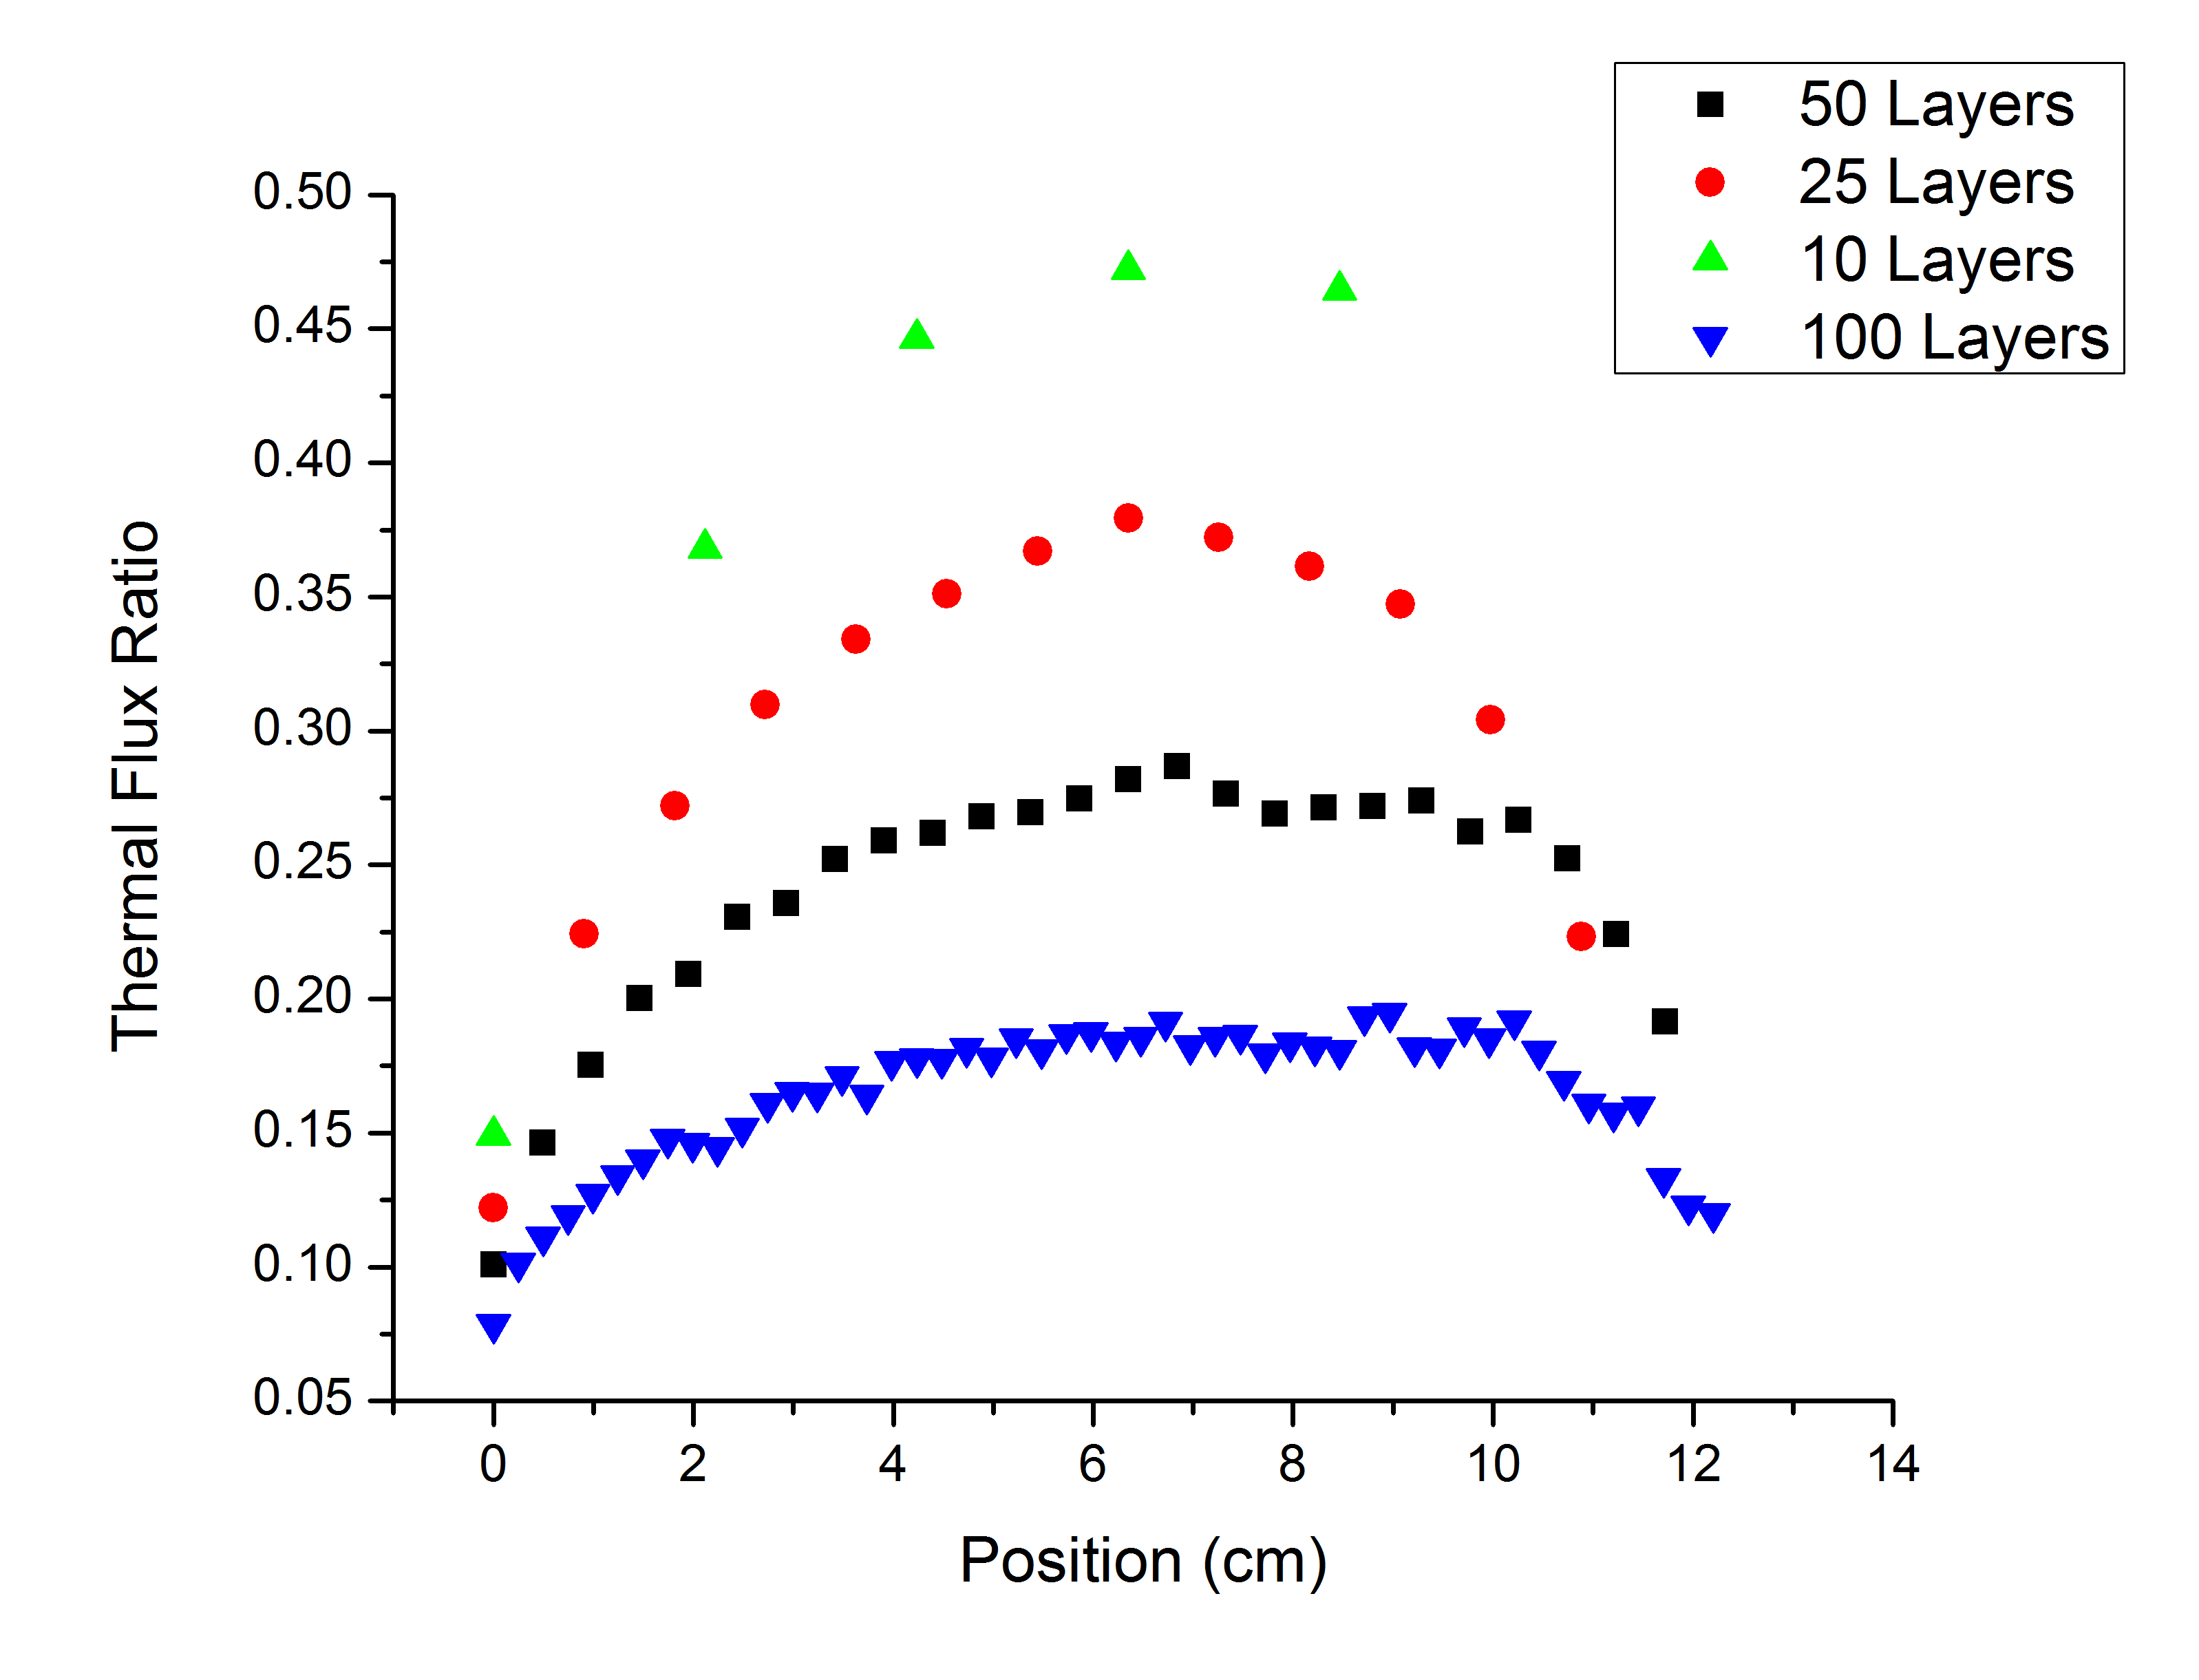
\includegraphics[width=\textwidth]{ThermalFluxRatioAltLayers}
	\caption{Fraction of the neutron flux that is thermalized through a alternating detector and moderator layered RPM.  The low thermal fluxes result in a poor utilization of the high thermal cross section of \iso[6]{Li}.}
	\label{fig:AltLayerThermalNeutronFraction}
\end{figure}
Several different strategies can then be used to optimize the geometry to ensure effective utilization of the thermal cross section of the absorber material.


\subsection{Proposed Work}
The cost of a radiation portal monitor can be broken into the material cost, the cost of the associated electronics, and the assembly cost.
The material cost consists of the neutron absorbing material, the cost of any neutron moderator materials, and the cost of any encasing material. 
It is thought that the \iso[6]{Li} will dominate the material cost.
As the detector is a scintillation based detector the electronics will consist of photomultiplier tubes and the associated electronics to create the necessary readout.
In addition there is also a cost to assemble the detector which will depend primarily on the number of components to assemble.

It is then proposed to design a methodology for the optimization of layered detectors that satisfy the criteria set forth in \autoref{tab:DHSCritera}.
The completed work will consist of a robust code base that can be easily adapted to different materials that can be easily optimized.
The utilization of this toolkit will yield a detector design that satisfies the DHS DNDO criteria while minimizing the mass of neutron absorber used in the detector.
\todo[inline]{It would be better if I could reformulate it to minimize the total cost of the detector - because in a carborane system it might not be the case that carborane scintillator dominates the detector cost}

\subsection{Methodology}
The proposed research laid out above will be accomplished using MCNPX to model the performance of a detector and genetic algorithms to search the possible candidate space of detector designs for the optimal design.
MCNPX was chosen as the neutronics simulation code because it is a well validated code that has been used by others to simulate RPM detector performance.
Previous experience has shown that the run time of the code is not that prohibitive (around \SI{1.72}{\minute}), but future enhancements might be to implement the geometry in a 1D transport code for significant speedup.
The MCNPX modeling is described in more detail in \autoref{sec:MCNPDetectorModelingMethod}
The optimization of the detector was chosen to be formulated as finding the detector design that maximizes the count rate per mass of absorber while still meeting the minimum count rate.
If the thickness of the RPM (\SI{12.7}{\cm}) is divided into equal slices where a slice can either contain a detector (\verb+1+) or moderator (\verb+0+) genetic algorithms can be used to effectively search this complex hypothesis space of possible detector designs for one that uses the minimum mass of absorber while still meeting the count rate criteria.
An overview to the genetic algorithm optimization is provided in \autoref{sec:GeneticAlgoSearchMethod}.
\subsubsection{MCNPX Detector Modeling}
\label{sec:MCNPDetectorModelingMethod}
The performance of films is simulated in MCNPX, a Monte Carlo transport code\cite{pelowitz_mcnpx_????}.
The geometry is as in the PNNL reports, namely a nano-gram of \iso[252]{Cf}  encased in \SI{0.5}{\cm} of lead and \SI{2.5}{\cm} of HDPE. 
The size of the RPM8 is \SI{12.7}{\cm} deep, by \SI{30}{\cm} wide and \SI{2}{\m} tall.

The interaction rate is calculated using the a cell flux tally in MCNPX and a tally multiplier card.
The tally multiplier card (FMn) is used to calculated any quantity of the form \eqref{eqn:FMCardForm} \cite{pelowitz_mcnpx_????}
\begin{align}
  \label{eqn:FMCardForm}
  I &= C\int\phi(E)\Re_m(E)dE
\end{align}
where \definevar{$I$}{Interaction rate}, \definevar{$\phi(E)$}{Energy dependent fluence} , \definevar{$\Re_m(E)$}{Response function operator} and $C$ is an arbitrary scalar for normalization.
An general example of the use of the FM card is shown in Listing \ref{lst:GeneralFMExample}, which is taken from the MCNPX manual \cite{pelowitz_mcnpx_????}.
% See pg. 4-41 of the MCNP manual
\begin{lstlisting}[caption={[Example usage of the FM card]Example usage of the FM card to calculate the number of reactions per \si{\cm\cubed} of type R in cell 8 of material M. The normalization is by atomic density, signified by the -1},label={lst:GeneralFMExample}]
F104: N 8
FM104 -1 M R
\end{lstlisting}

The reaction rate $\iso[6]{Li}\left(\text{n},\text{t}\right)\alpha$ can be calculated by then applying the appropriate input for the FMn card and using an F4 card to calculate $\phi(E)$.
It should be noted that depending on the form of the cell flux card it may be necessary to normalize by the volume of the cell, $\forall$.
\nomenclature{$\forall$}{Volume of the cell}

This is shown in Listing \ref{lst:InteractionRateRPM}, where the reaction number is 105 and the material number of the detector is 3.
The interaction rate in a simulated RPM8 replacement detector is calculated in a similar manner as the simulation of the measured detectors; the interaction rate as computed by the \verb+FMn+ is multiplied by the source strength and volume if necessary.
An example of the MCNPX input cards is shown in Listing \ref{lst:InteractionRateRPM}.
Given that there the thermal response is not desired, there is no need to subtract out the differences between the spectra, and the interaction rate is simply \eqref{eqn:RPM8InteractionRate}.
Note that in this calculation the source strength is set to be \SI{1}{\nano\gram} \iso[252]{Cf}, which has a neutron emission rate of \SI{2.3E3}{neutron\per\second}.
This is in accordance with the direct evaluation of the PNNL criteria, which require a absolute neutron count rate of \SI{2.5}{count\per\second\per\nano\gram\iso[252]{Cf}}.
\begin{lstlisting}[caption={[RPM8 ${}^{6}\text{Li}\left(\text{n},\text{t}\right)\alpha$ Reaction Rate]RPM8 ${}^{6}\text{Li}\left(\text{n},\text{t}\right)\alpha$ Reaction Rate. The detector is all of the layers of cell 500 inside universe 610. This tally is multiplied by an SD card to normalize by the volume},label={lst:InteractionRateRPM}]
FC4 (n,t) Reactions in Thin Film (Neutron Detector)
F4:n (500<610)
SD4 1
FM4 -1 3 105
\end{lstlisting}
\begin{align}
  \label{eqn:RPM8InteractionRate}
  I_{\text{sim}} &= S_0 I \\
  &= \SI{2.3E3}{neutron\per\second} I
\end{align}

$I_{\text{sim}}$ provides the total number of simulated neutron interactions in the detector.
However, not all of these interactions will lead to counts above the pulse height discriminator setting necessary for meeting the gamma intrinsic efficiency.
This is corrected for by scaling $I_{\text{sim}}$ by the fraction of counts, $\eta$, that occur above the gamma LLD \eqref{eqn:FractionOfCountsDefination}, \eqref{eqn:RPMCountRate}.
\begin{align}
  \label{eqn:FractionOfCountsDefination}
  \eta \equiv \frac{\int_{MLLD}^\infty p(x)dx}{\int_0^\infty p(x)dx}
\end{align}
\nomenclature{$p(x)$}{Measured spectra, as a function of channel number}
\begin{align}
 \label{eqn:RPMCountRate}
 \text{Count Rate} &= I_{\text{sim}} \eta
\end{align}

\subsubsection{Genetic Algorithm Search}
\label{sec:GeneticAlgoSearchMethod}
Genetic algorithms provide a search method analogous to biological evaluation. 
Rather than following a gradient of a response function, genetic algorithms generate possible hypothesis by repeatedly applying genetic operators (mutation and recombination) to the best currently known hypothesis for the generation of subsequent populations of hypothesis. 
In this way the search space of candidate hypothesis (possible detector designs) is searched to identify the best hypothesis; the design that uses the least amount of \iso[6]{Li} while meeting the criteria. 
The genetic algorithm typically consist of four tasks: 
\begin{enumerate}
  \item creating an initial population, 
  \item evaluating that populations fitness, 
  \item selecting members of the current population to breed, and 
  \item applying genetic operators to the selected members to breed the new population. 
\end{enumerate}	
This is completed until either a maximum generation is reached or the desired fitness is achieved.
\begin{figure}
\begin{algorithmic}
  \WHILE{$error>goal$}
		\FORALL{$p \in P$}
			\STATE{Compute fitness}
		\ENDFOR
		\FORALL{$p \in P$}	
			\STATE{Choose individuals based on fitness}
			\STATE{Select individuals for next population}
			\STATE{Crossover selected individuals}
			\STATE{Mutate selected individual}
		\ENDFOR
	\ENDWHILE
\end{algorithmic}
\caption{Genetic Program Outline}
\label{AlgoOutline}
\end{figure}

PyEvolve is a free Python implementation of genetic algorithms.
The PyEvolve toolkit was chosen for this work because of pythons scripting ability as well as the visualization and performance indicators of the PyEvolve toolkit.
In order to decrease the computational time is it proposed to use memoization to store detector solutions, where the bit string representation of the geometry is used as a hash for a dictionary.  
In addition, where possible multi-threading will be utilized.

%%%%%%%%%%%%%%%%%%%%%%%%%%%%%%%%%%%%%%%%%%%%%%%%%%%%%%%%%%%%%%%%%%%%%%%%%%
%                                                      									 %
%                  		  	RPM Light Collection                           %
% 									                                                     %
%%%%%%%%%%%%%%%%%%%%%%%%%%%%%%%%%%%%%%%%%%%%%%%%%%%%%%%%%%%%%%%%%%%%%%%%%%
\section{RPM Light Collection Performance}
\label{sec:RPMLCP}

There is no assurance that the detectors designed based on interaction rate would be feasible to construct; due to their low light output and opaqueness collecting the light from scintillation events would be extremely difficult.  
Additional simulation work then needs to be completed to ensure that a RPM in the layered detector design has a realistic method of collecting the light emitted from the scintillation events.
Light transport modeling provides a way to calculate the performance of such a design while providing insights for the improvement of a detector design.

Several previous authors have used the GEANT4 toolkit to simulate the light collection efficiency of their detector designs.
In PNNL 14283 the authors looked at a variety of different PMT placement and detectors designs to increase the light output of a detector in the Advanced Large-Area Plastic Scintillators (ALPS) project \cite{pnnl_14283}.
The authors found that for a \SI{127}{\cm} by \SI{57}{\cm} by \SI{5}{\cm} slab of BC-408 wrapped in a loose foil of 85\% reflectivity that the light output could be almost doubled by doubling the number of PMT's.
These results are summarized in \autoref{tab:PNNLLightCollectionEfficiency}.
\begin{table}
  \centering
  \caption[PNNL Light Collection Efficiencies]{Light collection efficiencies of several detector designs simulated by PNNL\cite{pnnl_14283}.}
  \label{tab:PNNLLightCollectionEfficiency}
  \begin{tabular}{c|c c}
  \toprule
  & \multicolumn{2}{c}{Light Collection Efficiency} \\
  Number of PMTs  & 2-in PMT & 5-in PMT \\
  \midrule
  2 & 7.0\% & 18.8\% \\
  4 & 13.3\% & 30.7\ \\
  6 & 18.4\% & 40.2\% \\
  \bottomrule
  \end{tabular}
\end{table}
In addition, other authors have reported on the simulation performance of a light guides and photon attenuation using the GEANT4 toolkit.
An overview of the light transport and scintillation processes available in GEANT4 is presented in \cite{riggi_introducing_2011}.
The authors also simulated a \SI{1}{\m} by \SI{1}{\cm} by \SI{1}{\cm} plastic strip in order to calculate the photon attenuation in the plastic.
Two orders of magnitude drop in the number of photons was calculated for photons collected \SI{90}{\cm} from the distance of emission, and was highly dependent of the reflectivity of the material encasing the plastic strip\cite{riggi_introducing_2011}.
Polymeric detectors containing PPO/POPOP as the fluor have also been modeled for the light transport with GEANT4\cite{5485130}.
This provides a measure of confidence that the films fabricated at the University of Tennessee containing PPO/POPOP can also be simulated without undo burden in finding light transport properties.

\subsection{Proposed Work}
It is proposed to simulate the neutronics, energy deposition, and light transport and collection of the optical photons with the GEANT4 toolkit to ensure that the proposed detector designs will be feasible. 
This will then have two parts:
\begin{enumerate}
  \item the fabrication and simulation of detectors whose performance can be measured in the laboratory, and
  \item the simulation of a RPM in the geometry specified by the neutronics calculations.
\end{enumerate}
It is also proposed to explore the design space of the light collection instrumentation, where such design options include
\begin{itemize}
  \item the use of a wavelength shifter (WLS) to increase the detected optical photons by decrease the optical photons absorbed in the light guide,
  \item the design of a light guide to enhance the photons reflected towards the PMT,
  \item the application of different light reflection techniques (air gap, Teflon tape, aluminized mylar) to enhance the light collection, and
  \item the placement of PMT's for their effective utilization.
\end{itemize}
The developed GEANT4 application will then have the ability to fully simulate the performance of a replacement RPM.

\subsection{Methodology}
The full simulation of the light transport of the RPM will be completed in with the GEANT4 toolkit.
GEANT4 offers three example simulations for generation and tracking of optical photons (\verb+ExampleN06+, \verb+extended/LXe+, and \verb+extended/WLS+).
These examples will be adapted for the purposes of this simulation.
However, it should be noted that the \verb+LXe+ and \verb+WLS+ utilize a sensitive detector which kills tracks, and for the purposes of the simulation of the RPM this will not be implemented.

The validation of the GEANT4 simulations will be completed with the fabrication of a 4 inches by 6 inches layered detector to allow the toolset to be benchmarked against measurements.
Detectors of various materials (boron loaded plastic, lithium loaded polymers, and LiF/ZnS(Ag)) will be tested to avoid a basis in the simulation parameters.
Where possible, the optical parameters of the materials will be taken from the literature.
However, it they cannot be found a similar material for which the property is know will be substituted.
In addition, rather than providing reflectivity parameters for each material, a model of optical surface will be used according to the work of Janecek\cite{5485130}. 

The GEANT4 light transport simulation code base will be written such that bit-string geometries from genetic algorithm optimization can be directly implemented.
With this formulation it will be possible to reuse the genetic algorithm optimization code base, while additionally providing a validation of the GEANT4 neutronic calculations against the MCNPX.
  % Proposal and Methodol
    \chapter{Summary, Deliverables and Timetable}
\label{ch:SummaryDeliverables}
\section{Summary}
Defense against nuclear terrorism relies upon the ability to accurately detect and identify Special Nuclear Material (SNM).
The current standard for neutron detection in portal monitors is \iso[3]{He}, which is a diminishing resource. 
A significant amount of research is then focused on developing new (or optimizing an existing) neutron detection system to serve as a replacement RPMs.
Previous work by this author focused on the characterization of replacement polymeric thin film detector technologies for RPMs.  
The proposed work will focus on designing a framework for determining an optimized detector design for replacement RPMs based on polymeric thin films.
This work will be novel in its utilization of high fidelity energy deposition to explain the origins of neutron-gamma discrimination through the range of secondary electrons from the neutron and photons reactions in their subsequent energy deposition.
The neutronic performance of a film will then be assessed by calculating the performance of a full scale replacement RPM in the test environment with MCNPX.
Non-linear search techniques will then be used to find the optimal geometry of the MCNPX model of the detector that best utilizes the neutron absorber.
Finally, the scintillation light from the detectors will be simulated with the GEANT4 toolkit, and the performance of the detector based upon the collected light signal reported.
Different light collection strategies will be employed to maximize the light collection efficiency and minimize the cost of electronics necessary for the detector.


\section{Delerivables and Timetable} 
The proposed optimization strategy will first optimize on the microscopic domain of the energy deposition of a single layered detector (supporting the simulations with measurements) and then optimize the performance on the macroscopic domain of a large area plastic scintillator detector.
What has been proposed is essentially an architecture for the optimization that can be broken down into modules.
For each of the subsystems, the developed code will be well documented in order to ensure that the toolkit is portable and with the ability to be extended.
In addition, self-contained repositories of the code base will be made available.
Doxygen, a standard tool for extracting documentation for annotated C++ sources will be used to develop HTML based documentation files and a project manual.
If time permits a tutorial will be developed to assist others in replicating this work.
Measurements made to validate the simulations will also be well documented, and hopefully self contained.
This is to ensure the portability of this work.
\autoref{fig:OptArc} is a flow chart of the proposed optimization process in which the energy deposition simulations influence the inputs of the neutronics modeling and the light transport simulations.
If either of these simulations indicate that the DHS/DNDO detector criteria will not be meet, it is then necessary to modify the detector thickness or material in order to design a detector that will meet the criteria. 
\begin{figure}
  \centering
  \includegraphics[width=0.75\textwidth]{optArch}
  \caption[Optimization Architecture]{Optimization Architecture.  The energy deposition module provides inputs into the MCNP neutronics model and the GEANT4 Light transport simulations. Parameters available for optimization are shown in yellow, while measurement feedback is shown in cyan.}
  \label{fig:OptArc}
\end{figure}

The timelines for the proposed work is presented in the following charts.
\autoref{fig:AdmTimeline} shows a broad overview of the project milestones and accomplishements.
In \autoref{fig:CompletedWorkTimeline} the energy deposition and neutronics optimization by genetic algothrims are shown.
Finally \autoref{fig:LightTransportTimeline} presents the timeline for simulation of light transport.
%%%%%%% ADMINISTRATIVE TIMELINE %%%%%
\begin{sidewaysfigure}
\begin{center}
\begin{ganttchart}[x unit=8.5mm,vgrid,time slot format=isodate,compress calendar,today=2013-08-05,today offset=.5,today label=Current Week,today rule/.style={draw=blue,ultra thick}]{2012-06-12}{2013-12-30}
\gantttitlecalendar{year} \\
\ganttgroup[progress=100]{Energy Modeling}{2012-06-15}{2013-06-01}\\
\ganttgroup[progress=90]{Neutronics Optimization}{2012-12-15}{2013-3-30}\\
\ganttgroup[progress=75]{GEANT4 Light Transport}{2013-4-1}{2013-9-1}\\
\ganttgroup[progress=50]{Write Up and Conclusions}{2013-7-1}{2013-10-1}\\
\ganttmilestone{Dissertation Proposal}{2013-8-9}\\
\ganttbar{Disserrtation Defense}{2013-10-1}{2013-11-1}\\
\ganttmilestone{Dissertation to Trace}{2013-11-27}\\
\ganttmilestone{Pass/Fail Form}{2013-11-27}\\
\end{ganttchart}
\end{center}
\caption{Proposed Adminstrative Timeline}
\label{fig:AdmTimeline}
\end{sidewaysfigure}
%%%%%%% COMPLETED WORK %%%%%%%
\begin{sidewaysfigure}
\begin{center}
\begin{ganttchart}[x unit=8.5mm,vgrid,time slot format=isodate,compress calendar,today=2013-08-05,today offset=.5,today label=Current Week,today rule/.style={draw=blue,ultra thick}]{2012-06-12}{2013-12-30}
\gantttitlecalendar{year} \\
\ganttgroup[progress=100]{Energy Modeling}{2012-06-15}{2013-06-01}\\
\ganttbar[progress=100]{Energy Deposition}{2012-06-15}{2013-4-15} \\
\ganttbar[progress=100]{Range}{2013-5-25}{2013-6-15} \\
\ganttmilestone{IEEE Secondary Electron Paper}{2013-06-15}\\
\ganttgroup[progress=90]{Neutronics Optimization}{2012-12-15}{2013-3-30}\\
\ganttbar[progress=100]{MCNP Neutronics}{2012-12-15}{2013-1-15} \\
\ganttbar[progress=100]{Scripted Input Decks}{2013-1-30}{2013-2-5}\\
\ganttlinkedbar[progress=90]{Genetic Algorthims}{2013-2-15}{2013-3-10}\\
\ganttmilestone{ANS Presentation}{2013-11-10}
\end{ganttchart}
\end{center}
\caption[Timeline of Completed Work]{Timeline of Completed Work.}
\label{fig:CompletedWorkTimeline}
\end{sidewaysfigure}
%%%% LIGHT TRANSPORT TIMELINE
\begin{sidewaysfigure}
\begin{center}
\begin{ganttchart}[x unit=8.5mm,vgrid,time slot format=isodate,compress calendar,today=2013-08-05,today offset=.5,today label=Current Week,today rule/.style={draw=blue,ultra thick}]{2012-06-12}{2013-12-30}
\gantttitlecalendar{year} \\
\ganttgroup[progress=75]{GEANT4 Validation}{2013-1-10}{2013-7-10}\\
\ganttbar[progress=100]{Flir Detectors}{2013-4-15}{2013-4-30}\\
\ganttbar[progress=100]{Fabrication of Detectors}{2013-1-10}{2013-7-10} \\
\ganttlinkedbar[progress=100]{GS20 Simulation}{2013-06-1}{2013-7-10}\\
\ganttlinkedbar[progress=80]{Layred Simulations}{2013-6-15}{2013-7-15}\\
\ganttgroup[progress=75]{GEANT4 RPM Light Transport}{2013-6-1}{2013-10-1}\\
\ganttbar[progress=50]{Prelimiary Simuation}{2013-7-1}{2013-7-20} \\
\ganttlinkedbar[progress=25]{Parameter Studies}{2013-8-1}{2013-9-1}\\
\ganttlinkedbar[progress=0]{Optimization}{2013-9-1}{2013-10-1}\\
\end{ganttchart}
\end{center}
\caption{Light Transport Timeline}
\label{fig:LightTransportTimeline}
\end{sidewaysfigure}
  % Deliverables
    %%%%%%%%%%%%%%%%%%%%%%%%%%%%%%%%%%%%%%%%%%%%%%%%%%%%%%%%%%%%%%%%%%%%%%%%%%
    % BIBLIOGRAPHY
    %%%%%%%%%%%%%%%%%%%%%%%%%%%%%%%%%%%%%%%%%%%%%%%%%%%%%%%%%%%%%%%%%%%%%%%%%%
    \bibliographystyle{apalike} % bibliography style - recommend using apalike-doi as it hyperlinks DOIs
    \bibliography{Bib} % Bib.bib included in the references directory
    %%%%%%%%%%%%%%%%%%%%%%%%%%%%%%%%%%%%%%%%%%%%%%%%%%%%%%%%%%%%%%%%%%%%%%%%%%%
    % APPENDIX - OPTIONAL - COMMENT IF NOT NEEDED
    %%%%%%%%%%%%%%%%%%%%%%%%%%%%%%%%%%%%%%%%%%%%%%%%%%%%%%%%%%%%%%%%%%%%%%%%%%%
    \makeAppendixPage   % make the appendix title page - can be edited in ut-thesis-template.tex
    \appendix
    %%%%%%%%%%%%%%%%%%%%%%%%%%%%%%%%%%%%%%%%%%%%%%%%%%%%%%%%%%%%%%%%%%%%%%%%%%%
%                                                                         %
%                              Start of Content                           %
%  This material was stolen from DetectorComparions located in:           %
% MillerResearch/documentation/ExperimentWriteUps                         %
%%%%%%%%%%%%%%%%%%%%%%%%%%%%%%%%%%%%%%%%%%%%%%%%%%%%%%%%%%%%%%%%%%%%%%%%%%%
\chapter{Measured Polymeric Film Detectors}
\label{chap:MeasuredFilmPerfomance}
\section{Introduction}

The potential application  of a material for use in a Radiation Portal Monitor (RPM) can be evaluated by measurements of the detector's sensitivity to gammas and the detector's response to neutrons.
A detector material might be a possible replacement if the there exists a neutron response that can be differentiated from photons for given sensitivity of gammas, namely \num{1E-6}.
A simple way to discriminate between gammas and neutrons is to use a pulse height discriminator, above which the detector detector will only record one photon out a million as a neutron.
Under this framework it is then possible to develop a mathematical lower level discriminator (MLLD) of the pulse height spectrum to function as this pulse height discriminator, and to then formulate the sensitivity requirement as the gamma intrinsic efficiency as a function of MLLD.
Six detectors (three boron loaded plastic scintillators, one LiF:ZnS(Ag) doped screen, GS20, a post processed composite PEN film, and a polystyrene) were then evaluated for their ability to perform in a RPM. 
The thickness of these detectors and mass of the absorber are shown in \autoref{tab:PhysicalProperties}.
\begin{table}
\centering
\caption[Detector Physical Characteristics]{Physical characteristics of the detector.}
\label{tab:PhysicalProperties}
  \begin{tabular}{p{6cm}| m{2cm} m{2cm} p{2.5cm}}
  \toprule
    & Absorber & Thickness &  Mass Absorber (mg) \\
    \midrule
    EJ 254 2.5\% & \iso[10]{B} & 1/4" & 59.5 \\
    EJ 254 1\% & \iso[10]{B} & 1/4" & 23.8 \\
    EJ 254 5\% & \iso[10]{B} & 3/4 & 356.1 \\
    EJ 425 HD2-PE & \iso[6]{Li} & \SI{0.1}{\mm} & 17.5 \\
    GS20 & \iso[6]{LI} & \SI{2}{\mm} & 155 \\
    Post Processed Composite PEN Film & \iso[6]{Li} & $\approx$ \SI{212}{\um} & 42.42 \\
    PS Film & \iso[6]{Li} & \SI{50}{\um} & 2.71 \\
    \bottomrule
  \end{tabular}
\end{table}

\section{Methods}
The neutron performance was determined by the \iso[252]{Cf} irridiator previously described, and the gamma source was the \iso[60]{Co} irridiator.
Due to the wide range of light output of these films it was necessary to use a two voltages (\SI{1000}{\volt} and \SI{1180}{\volt}) in order to capture the entire spectra on an ADC with a zero to \SI{10}{\volt} range with repeatable resolution.
However, a measurement of the GS20 peak in the lead well was always recorded which then allowed the spectra to be tied together based on this feature, as shown in \autoref{eqn:SettingScale}.
\begin{align}
  \label{eqn:SettingScale}
  \text{Feature at Setting A} &= \frac{\text{GS20 Peak at Setting A}}{\text{GS20 Peak at Setting B}} \;\; \left( \text{Feature at Setting B}\right)
\end{align}
The count rates are not scaled for gain and voltage settings as they should remain constant as long as counts are not pushed below the lower level discriminator or cause roll-off.
\subsection{Neutron Performance above Gamma Discriminator}
An accurate measure of the neutron performance above the pulse height discriminator is essential for the comparison between detector materials.
In \autoref{fig:GammaMLLDIntEff} it is shown that the location of the MLLD is a pretty stable measurement for PS films of a different thickness.
\begin{figure}
  \centering
  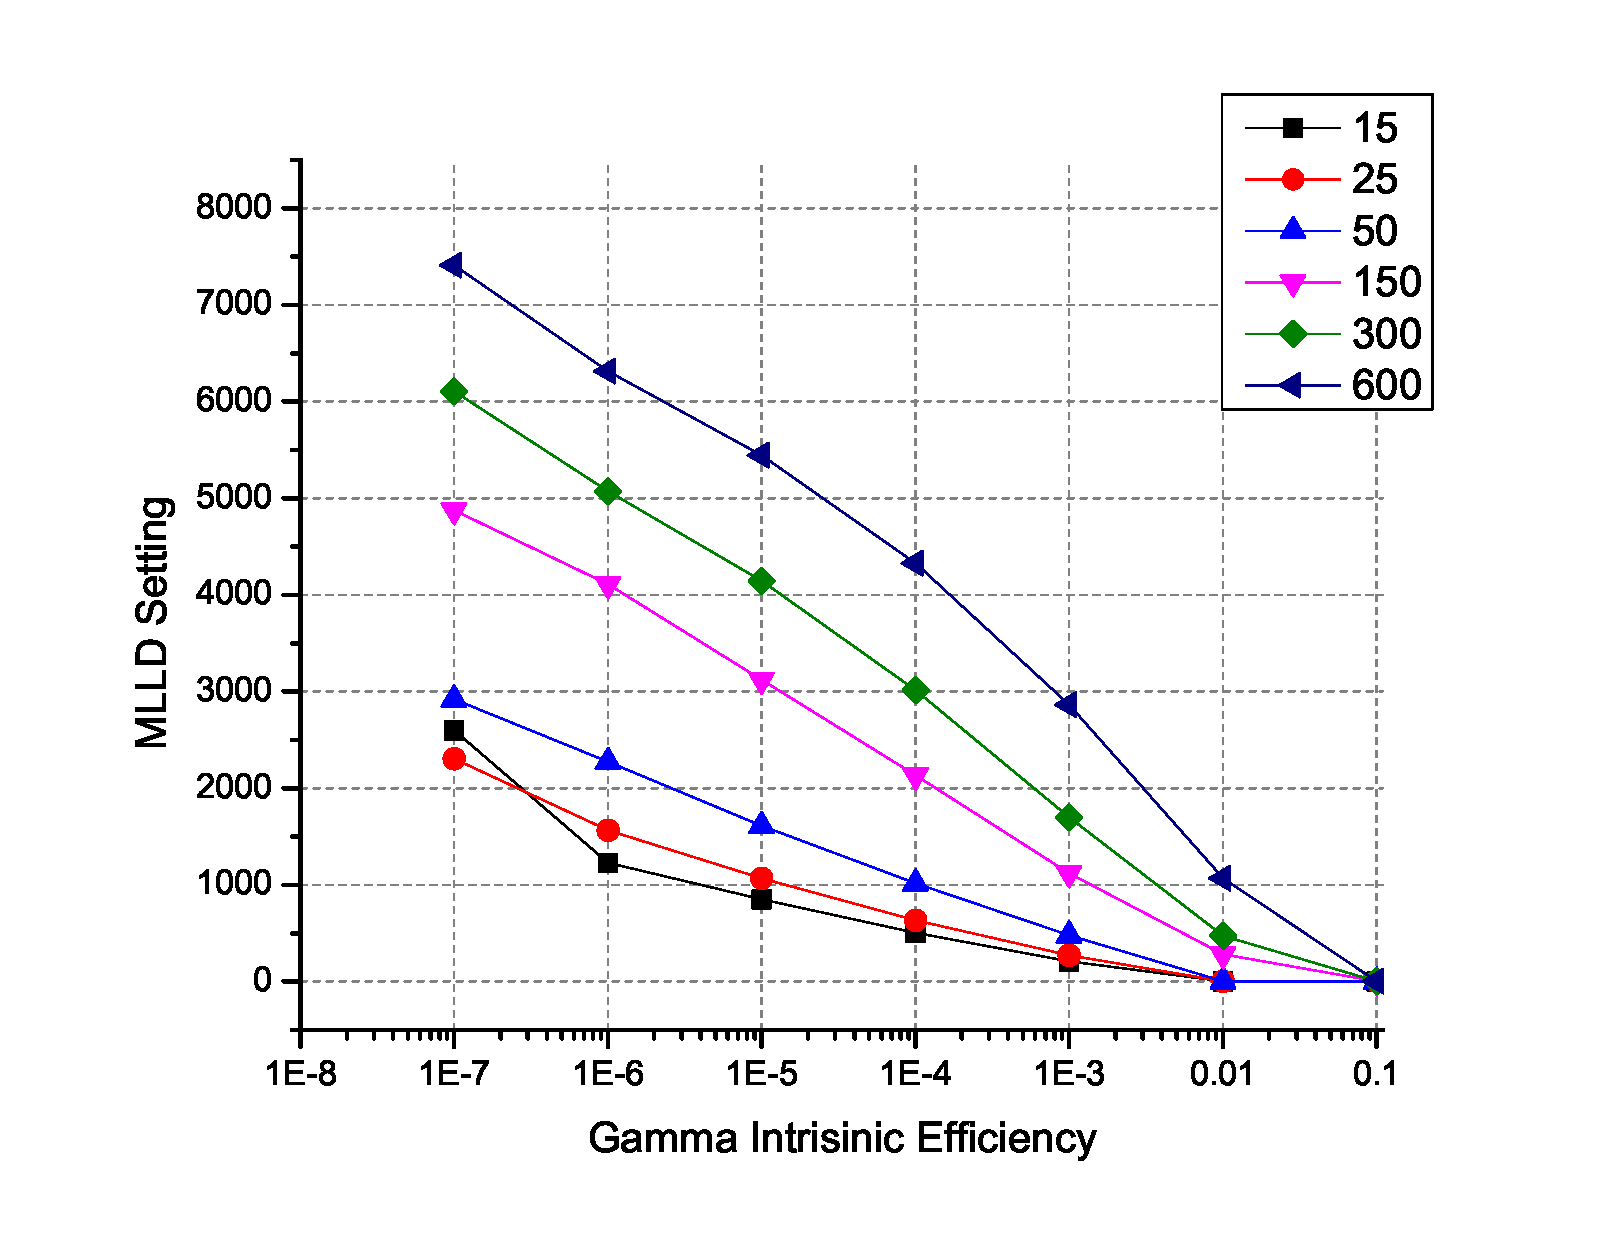
\includegraphics[width=\textwidth]{PS_IntEffMLLD_LiF}
  \caption[Stability of Lower Level Discriminator]{The mathematical lower level discriminator (MLLD) as a function of intrinsic effigies for 10\% PS films of various thickness. The linear nature suggest that the determination of the MLLD is repeatable.}
  \label{fig:GammaMLLDIntEff}
\end{figure}
However, in previous work which focused on using the fraction of neutron counts above the MLLD it was observed that the fraction (as it is normalized by the entire count rate) is very susceptible to sample to sample variations in the low energy channels.
Therefore, after extensive studies using the polystyrene matrix a more stable measure was found by simply integrating the counts in the neutron spectra above the MLLD and then normalizing by the mass of neutron absorber in the samples (\autoref{eqn:CountRateAbovePerMass}).
While this method does not have the errors associated with summing over the low channels, it does require an accurate measure of the mass of \iso[6]{Li} in the sample.
Alternative methods would also probably be stable, but they are not discussed here.
\begin{align}
\label{eqn:CountRateAbovePerMass}
\eta = \frac{\int_{\text{MLLD}}^\infty p(x)dx}{\text{Neutron Absorber Mass}}
\end{align}

\section{Results}
The following figures, \autoref{fig:Co60Spectra} and \autoref{fig:PbWellSpectra}, show the measured spectra of the detectors for neutrons and gammas.
It is clear that the EJ-254 (boron loaded plastic) detectors will have poor performance because of their large gamma response.
The EJ-426 (LiF:ZnS(Ag)) has the lowest response, and it is not clear if the tail of the spectra is due to actual counts or background.
In the neutron spectra it was decided to only plot the performance of the best EJ-254 (though \autoref{fig:EJ254Perf} display the performance of all EJ-254 films).
It is observed that the LiF:ZnS(Ag) is much brighter than the other films, and it is noted that the post processed composite PEN has a higher light output than the commercial EJ-254 (based on the peak location).
\begin{figure}
  \centering
  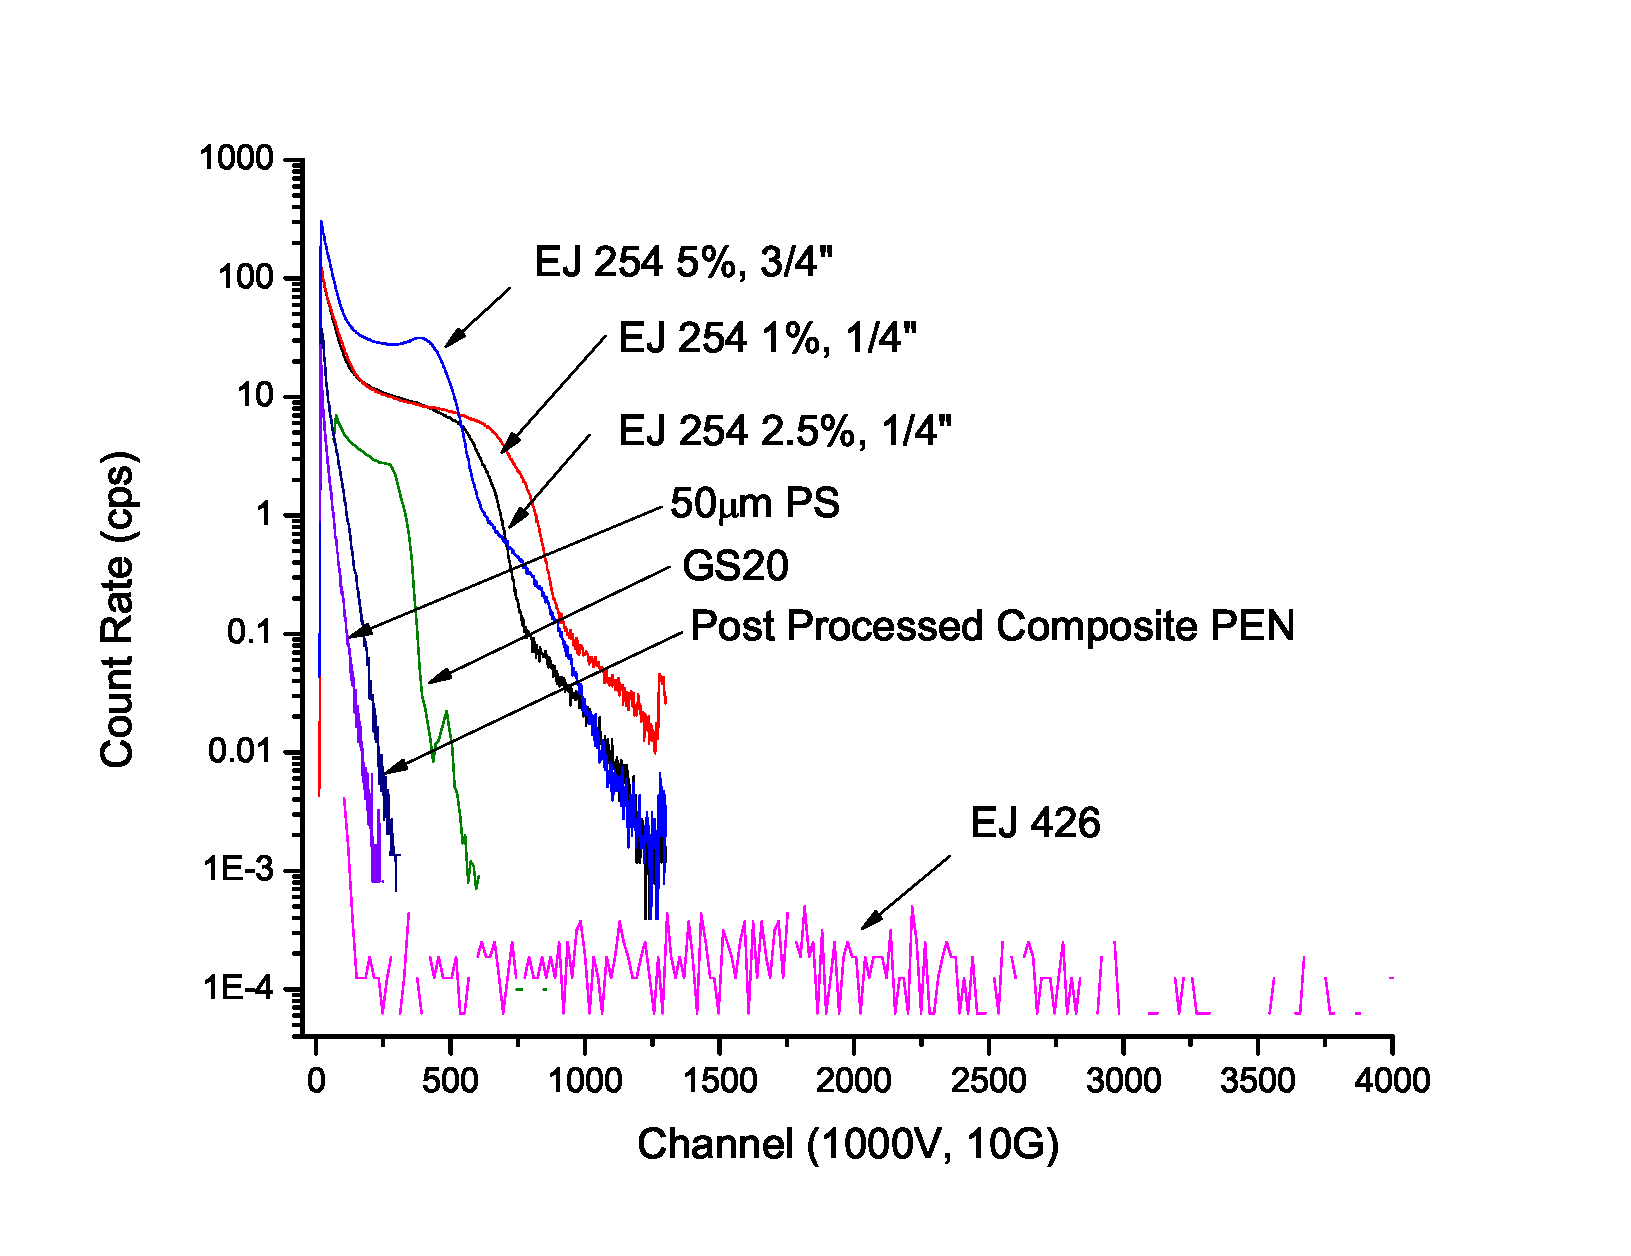
\includegraphics[width=\textwidth]{SampleComparions_Co60Spectra}
  \caption[Gamma Response of Measured Detectors]{Gamma Response from \iso[60]{Co} source of measured detectors.}
  \label{fig:Co60Spectra}
\end{figure}
\begin{figure}
  \centering
  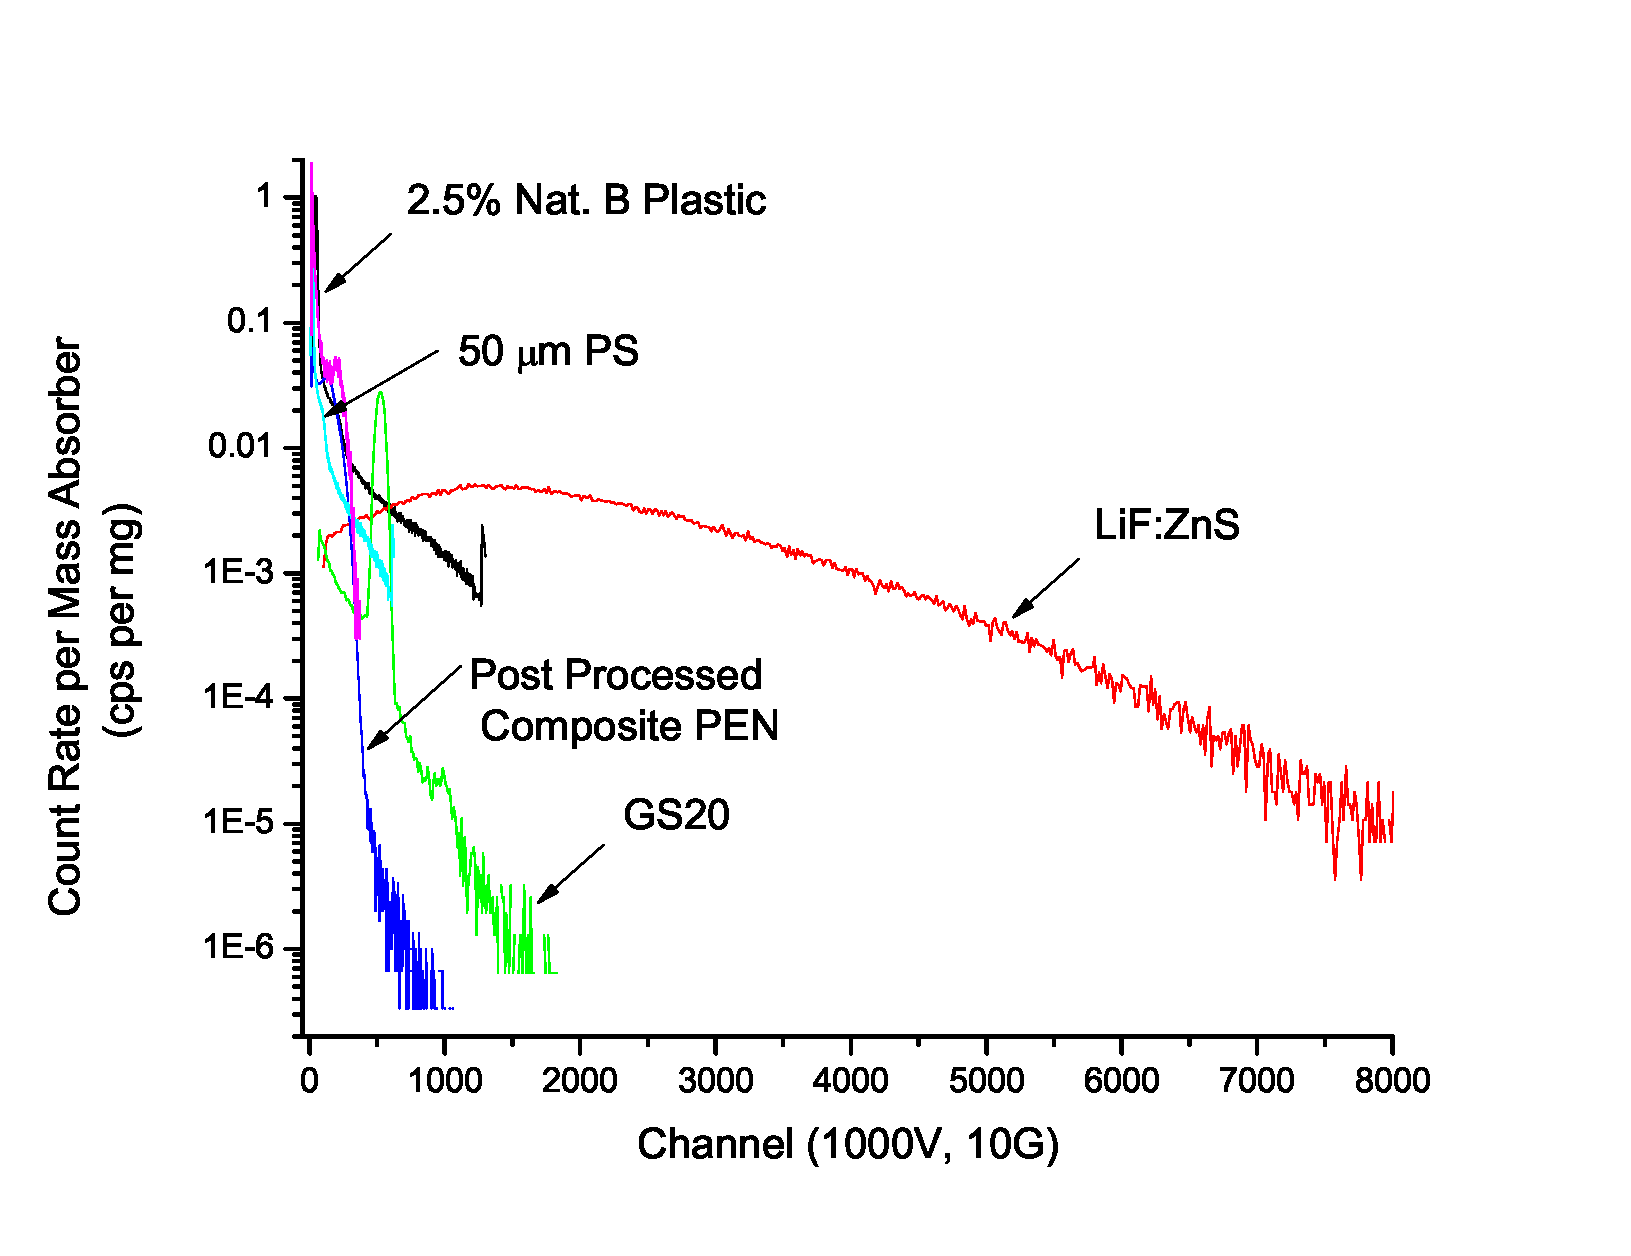
\includegraphics[width=\textwidth]{SampleComparison_PbCRperMg}
  \caption[Neutron Response of Measured Detectors]{Neutron Response (lead well) of the measured detectors. The count rate has been normalized by the mass of neutron absorber in the detector.}
  \label{fig:PbWellSpectra}
\end{figure}
The average channel number of the neutron and gamma spectra of each detector was calculated and are presented in \autoref{tab:AvgChNG}.
The average was computed for the neutrons in the thermal well to avoid the low energy channels from shifting the spectra away from any peak location.
It should be noted that for EJ-254 the low channel number average is correct; this feature was identified as the neutron peak.
Eljen publishes the light yield for the 1\% boron as 9,200 photons per MeVee, 8,600 photons per MeVee for the 2.5\% boron, and 7,500 photons per MeVee for the 5\% boron, and \autoref{tab:AvgChNG} shows agreement to these values.
C.W.E van Eijk has published the light yield of LiF:ZnS as 75,000 photons per MeVee, which is close to our measured value of 72,000 photons per MeVee.
\begin{table}
  \centering
  \caption[Average Channel Number of Gamma and Neutron Spectra]{Average channel number of gamma and the thermal neutron spectra.  The channel averages are scaled to 1,000V, 10G. The light yields are scaled to GS20 having 3,800 photons per MeV, and 6,250 photons per Neutron.}
  \label{tab:AvgChNG}
  \begin{tabular}{m{4cm}| m{2cm} m{2cm} |m{2cm} m{2cm}}
    \toprule
        &\multicolumn{2}{|c|}{Gamma}&\multicolumn{2}{|c}{Neutron}\\
        & Average Channel& Photons per MeVee & Average Neutron Channel & Photons per Neutron\\
    \midrule
    EJ 254 2.5\%, 1/4"&	183.41	&	8,100	&	54.06	&	640	\\
    EJ 254 1\%, 1/4"&	216.25	&	9,500	&	65.04	&	780	\\
    EJ 254 5\%, 3/4"&	176.49	&	7,800	&	39.56	&	479	\\
    EJ 426 HD2&	1636.53	&	72,000	&	2018.	& 	24,000	\\
    GS20 &	172.76	&	3800.00	&	524.10	&	6,250	\\
    Post processed Composite PEN & 41.11 & 1,800 & 142.01 & 1,700\\
    PS Film & 32.18 & 1,400 & 169.34 & 2,000 \\
    \bottomrule
  \end{tabular}
\end{table}
The count rates of the detectors are presented in \autoref{tab:CountRate} for both the thermal component as well as only in the lead well spectra.
\begin{table}
\centering
  \caption[Detector Count Rate]{Count rate of the detectors in the thermal spectra as well as the lead well spectra.  The final two columns are normalize by the mass of the absorber in the material. Significant self-shielding may exists in the the 5\% boron, 3/4" EJ-254.}
  \label{tab:CountRate}
  \begin{tabular}{m{4cm}| m{2cm} m{2cm} |m{2cm} m{2cm}}
  \toprule
    &\multicolumn{2}{|c|}{Count Rate}&\multicolumn{2}{|c}{Count Rate per Mass Absorber} \\
    &\multicolumn{2}{|c|}{(cps)}&\multicolumn{2}{|c}{(cps per mg)} \\
    & Thermal Neutrons &Lead Well & Thermal Neutrons & Lead Well\\
  \midrule
  EJ 254 2.5\%, 1/4"&	1104	&	1869	&	18.5	&	31.4	\\
  EJ 254 1\%, 1/4"&	447	&	1130	&	18.8	&	47.5	\\
  EJ 254 5\%, 3/4"&	1417	&	3415	&	3.98	&	9.59	\\
  EJ 42 6 HD2 \SI{0.1}{\mm}&	224	&	234	&	12.8	&	13.4	\\
  GS20 \SI{2}{\mm}&	328	&	412	&	2.12	&	2.66	\\
  Post processed Composite PEN $\approx$ \SI{212}{\um}&	322	& 227	&	5.35 &	7.60	\\
  PS, \SI{50}{\um}, 10\% LiF & 90.6 & 20.7 & 7.63& 33.4 \\
  \bottomrule
  \end{tabular}
\end{table}
\autoref{tab:DiscrimPreformance} shows the discrimination performance of the tested detectors, while \autoref{fig:DiscrimPerformance} plots the intrinsic efficiency (sensitivity) along with the neutron count rate, normalized by the absorber mass.
\begin{table}
  \centering
  \caption[Discrimination Performance]{Discriminator setting and count rate above the gamma intrinsic efficiency of \num{1E-6} for various detectors.}
  \label{tab:DiscrimPreformance}
  \begin{tabular}{m{5cm} | m{2cm} m{6cm}}
    \toprule
    &	MLLD Location	&	Count Rate above the intrinsic discriminator setting of \num{1E-6} per Absorber Mass (cps per mg)	\\
    \midrule
    EJ 254, 2.5\% B, 1/4"	&	1280	&	0.20	\\
    EJ 254, 1\% B, 1/4"	&	1300	&	0.05	\\
    EJ 254, 5\% B, 3/4"	&	1290		&	0.03	\\
    EJ 426 HD2, \SI{0.1}{\mm}&	3308		&	1.97	\\
    GS20, \SI{2}{\mm}	&	557		&	0.56	\\
    Post processed Composite PEN,\SI{212}{\um}, 25\% LiF	&	284	&	0.73	\\
    PS, \SI{50}{\um}, 10\% LiF & 223 & 2.15\\
    \bottomrule
\end{tabular}
\end{table}
\begin{figure}
  \centering
  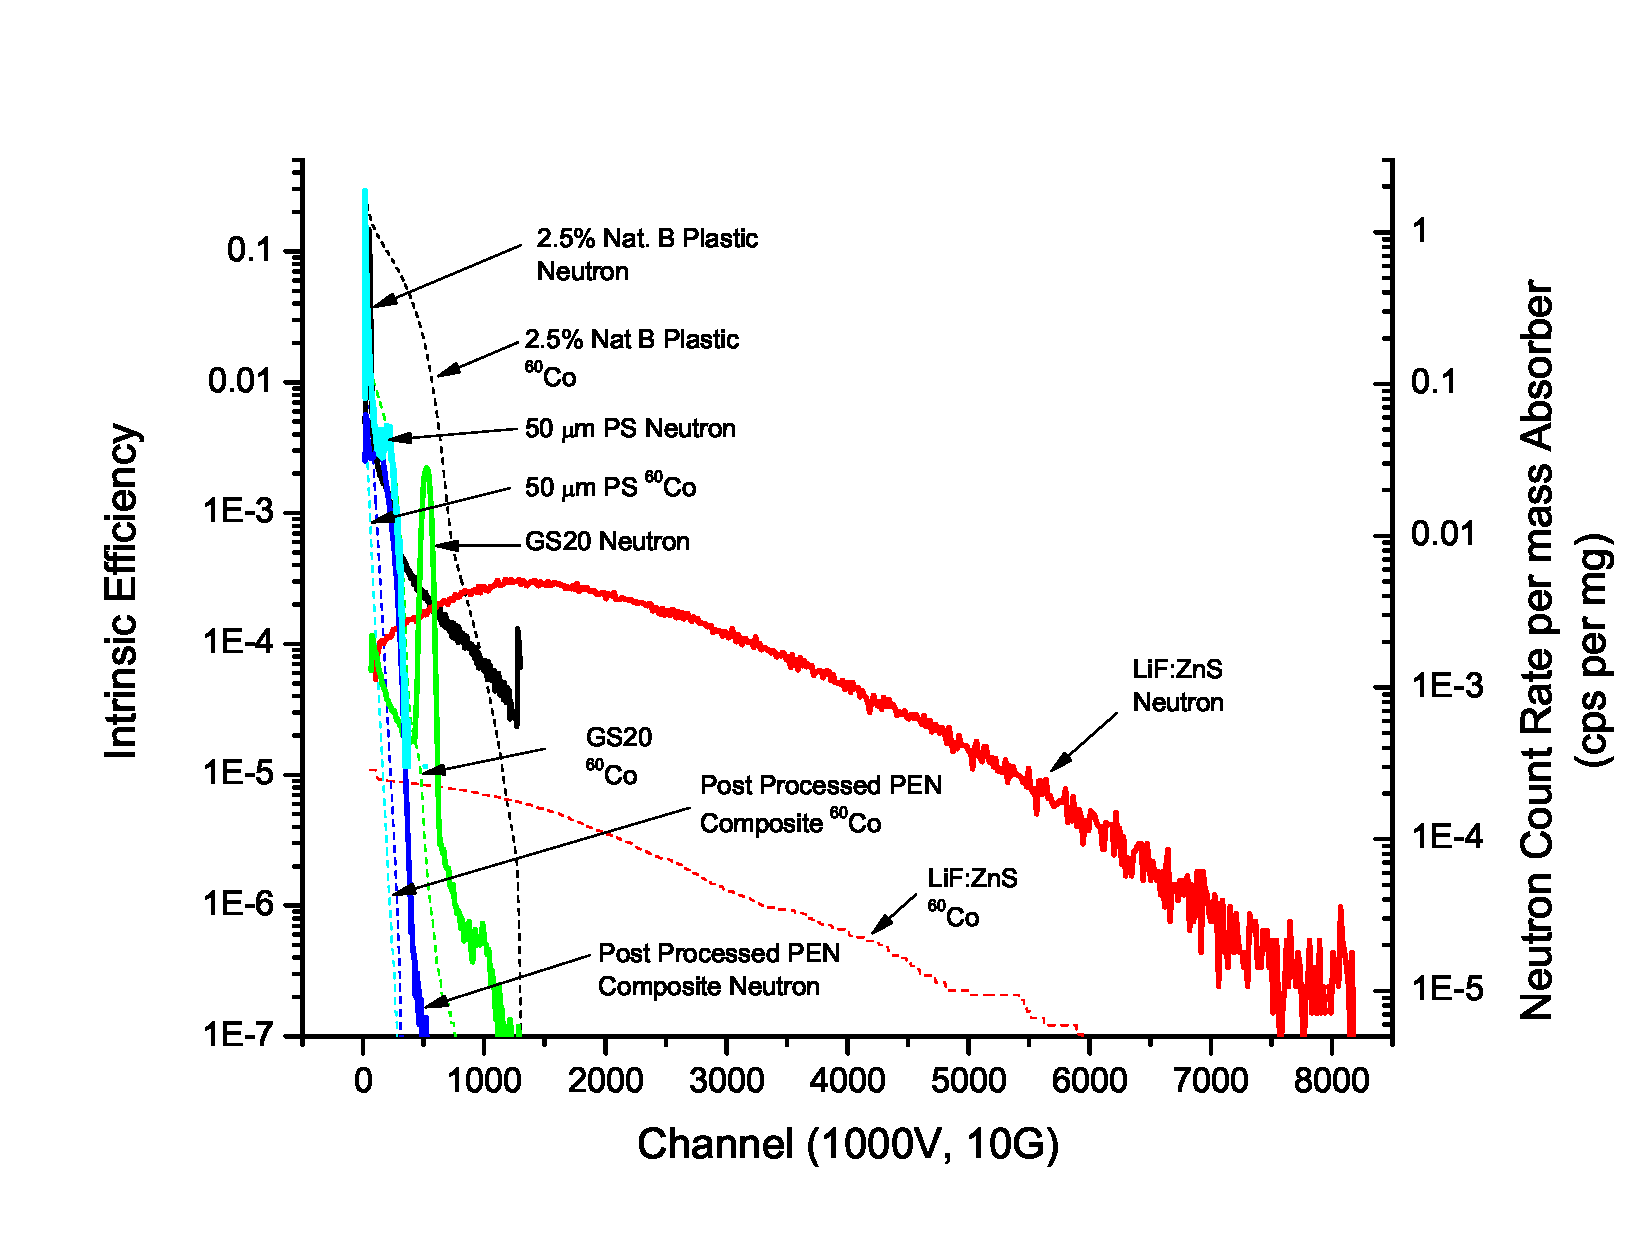
\includegraphics[width=\textwidth]{SampleComparison_IntEff_CR}
  \caption[Gamma Sensitivity and Neutron Response of Measured Detectors]{Gamma sensitivity (left axis, dashed lines) and neutron performance (right axis, solid lines) of measured detectors.  The neutron count rate above the gamma pulse height discriminator may be found by noting where the intrinsic efficiency crosses \num{1E-6} and then integrating the neutron spectra above it. The neutron spectra are from the lead well, and are normalized by the mass of absorber.}
  \label{fig:DiscrimPerformance}
\end{figure}
\autoref{fig:UTDetectorPreformance} demonstrates the performance of two detectors fabricated at UT (the PEN by Rohit Uppal and the PS by Andrew Mabe).
\begin{figure}
  \centering
  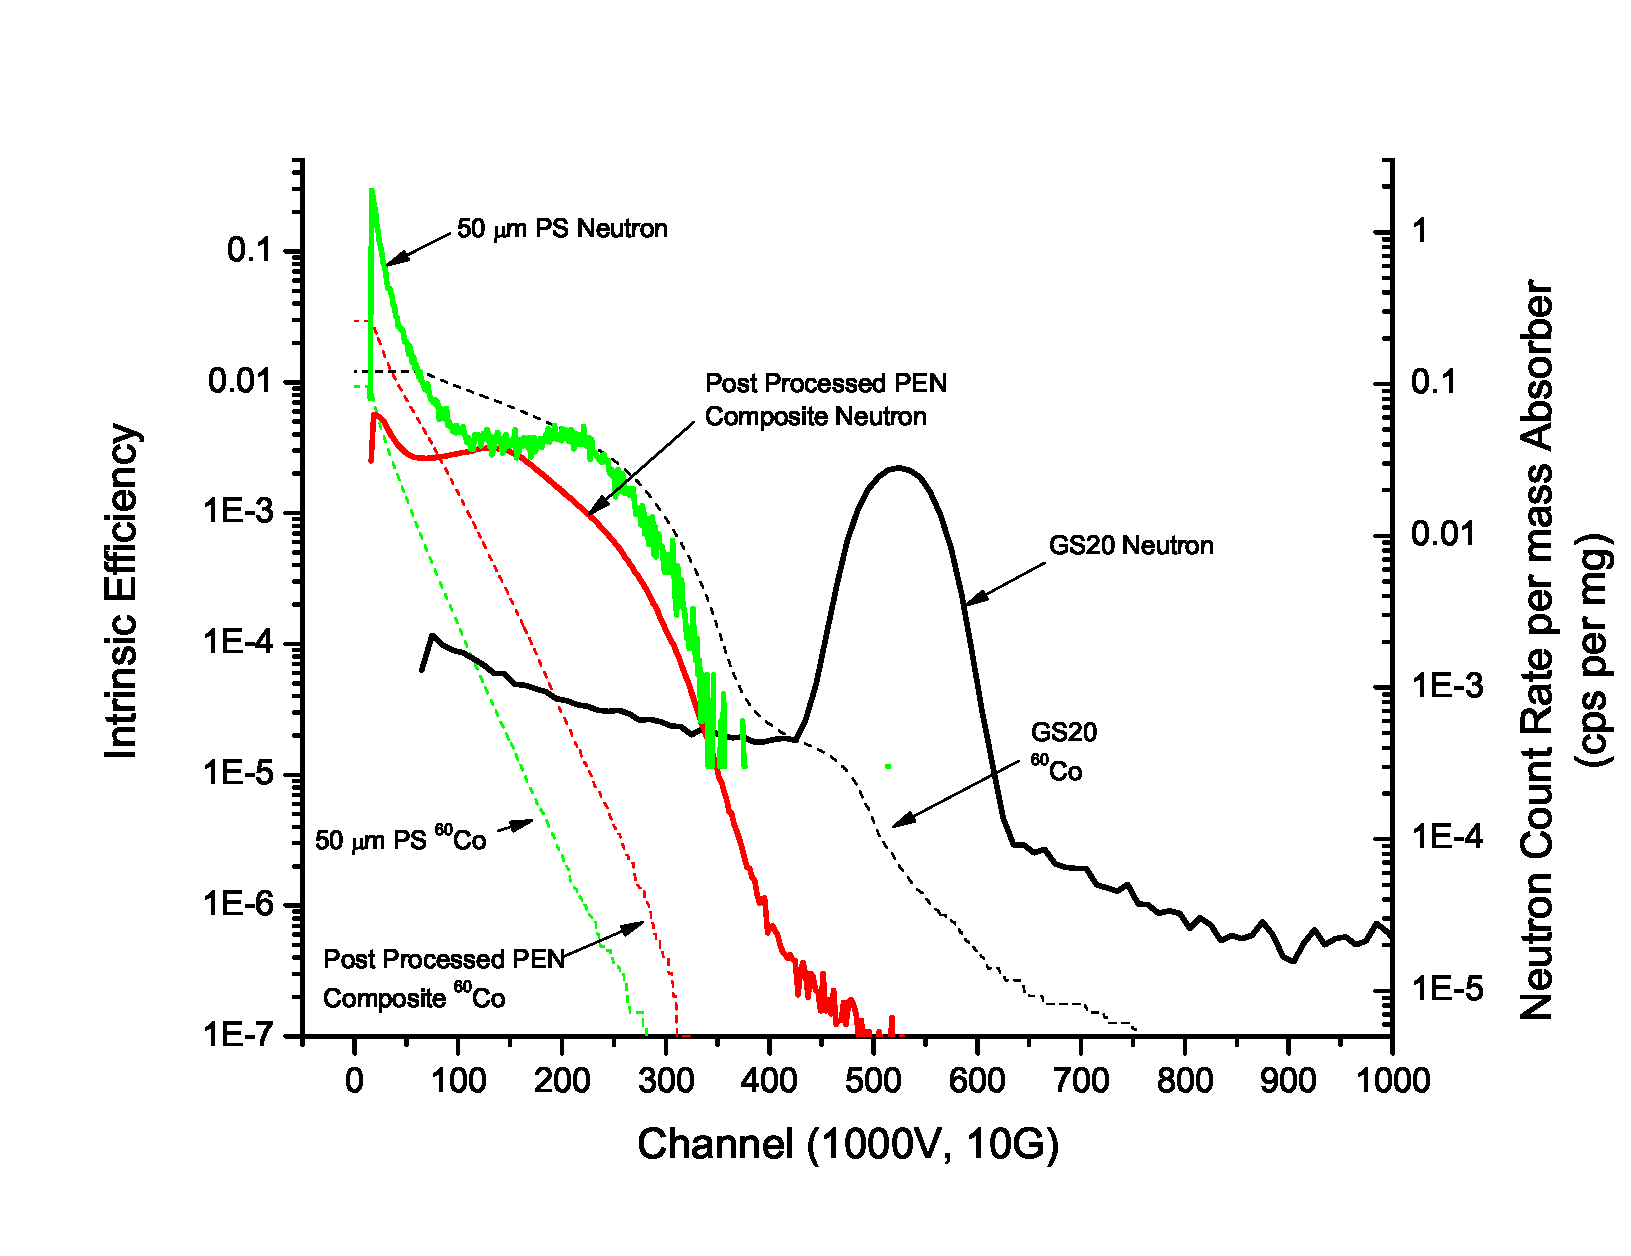
\includegraphics[width=\textwidth]{SC_UTDetectors_IntEff_CR}
  \caption[UT Fabricated Detector Performance]{Performance of a polystyrene and PEN film fabricated at UT compared to GS20.}
  \label{fig:UTDetectorPreformance}
\end{figure}

\subsection{Individual Detector Performance}
The performance of the individual detectors are shown in the separate figures to clearly illustrate important features.
\begin{figure}
  \centering
  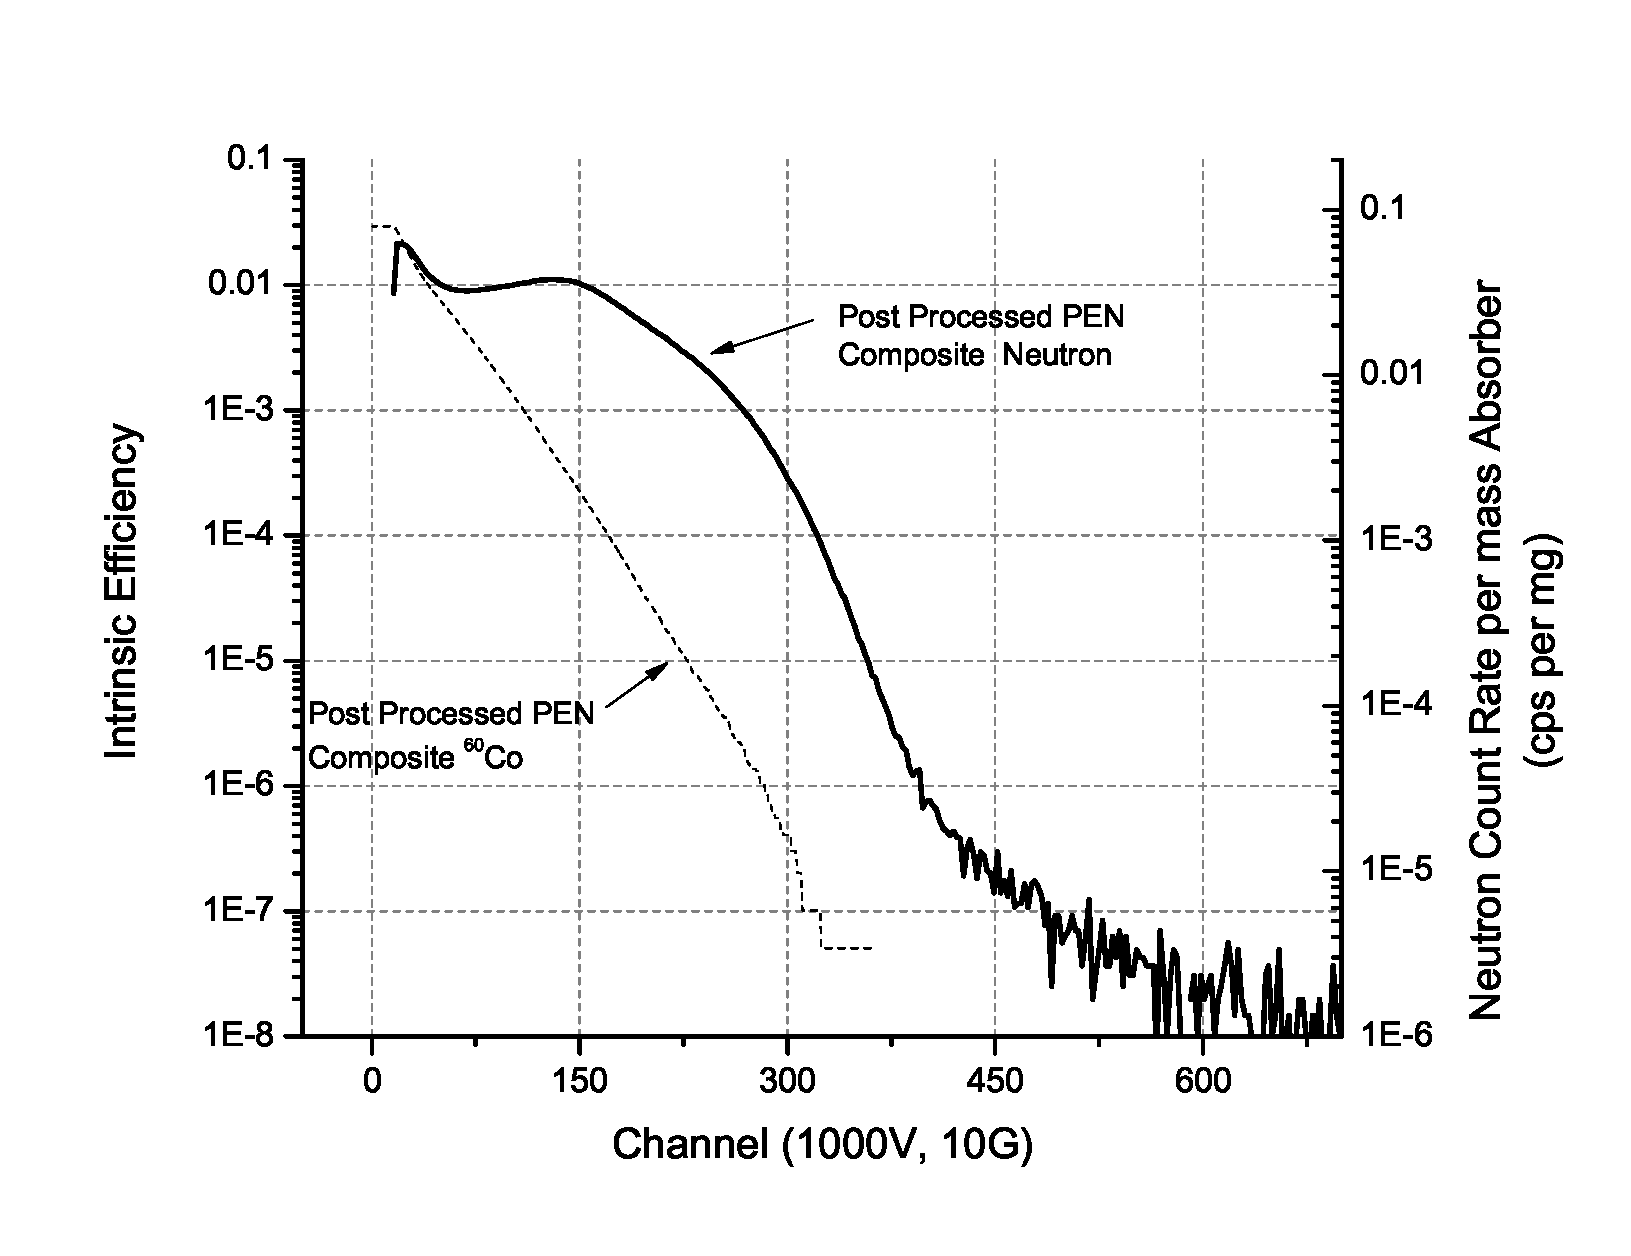
\includegraphics[width=\textwidth]{SC_ACPEN_IntEff_CR}
  \caption[Post processed Composite PEN Performance]{Performance of an Post processed Composite PEN Film (22 March Sample).}
  \label{fig:ACPENPreformance}
\end{figure}
\begin{figure}
  \centering
  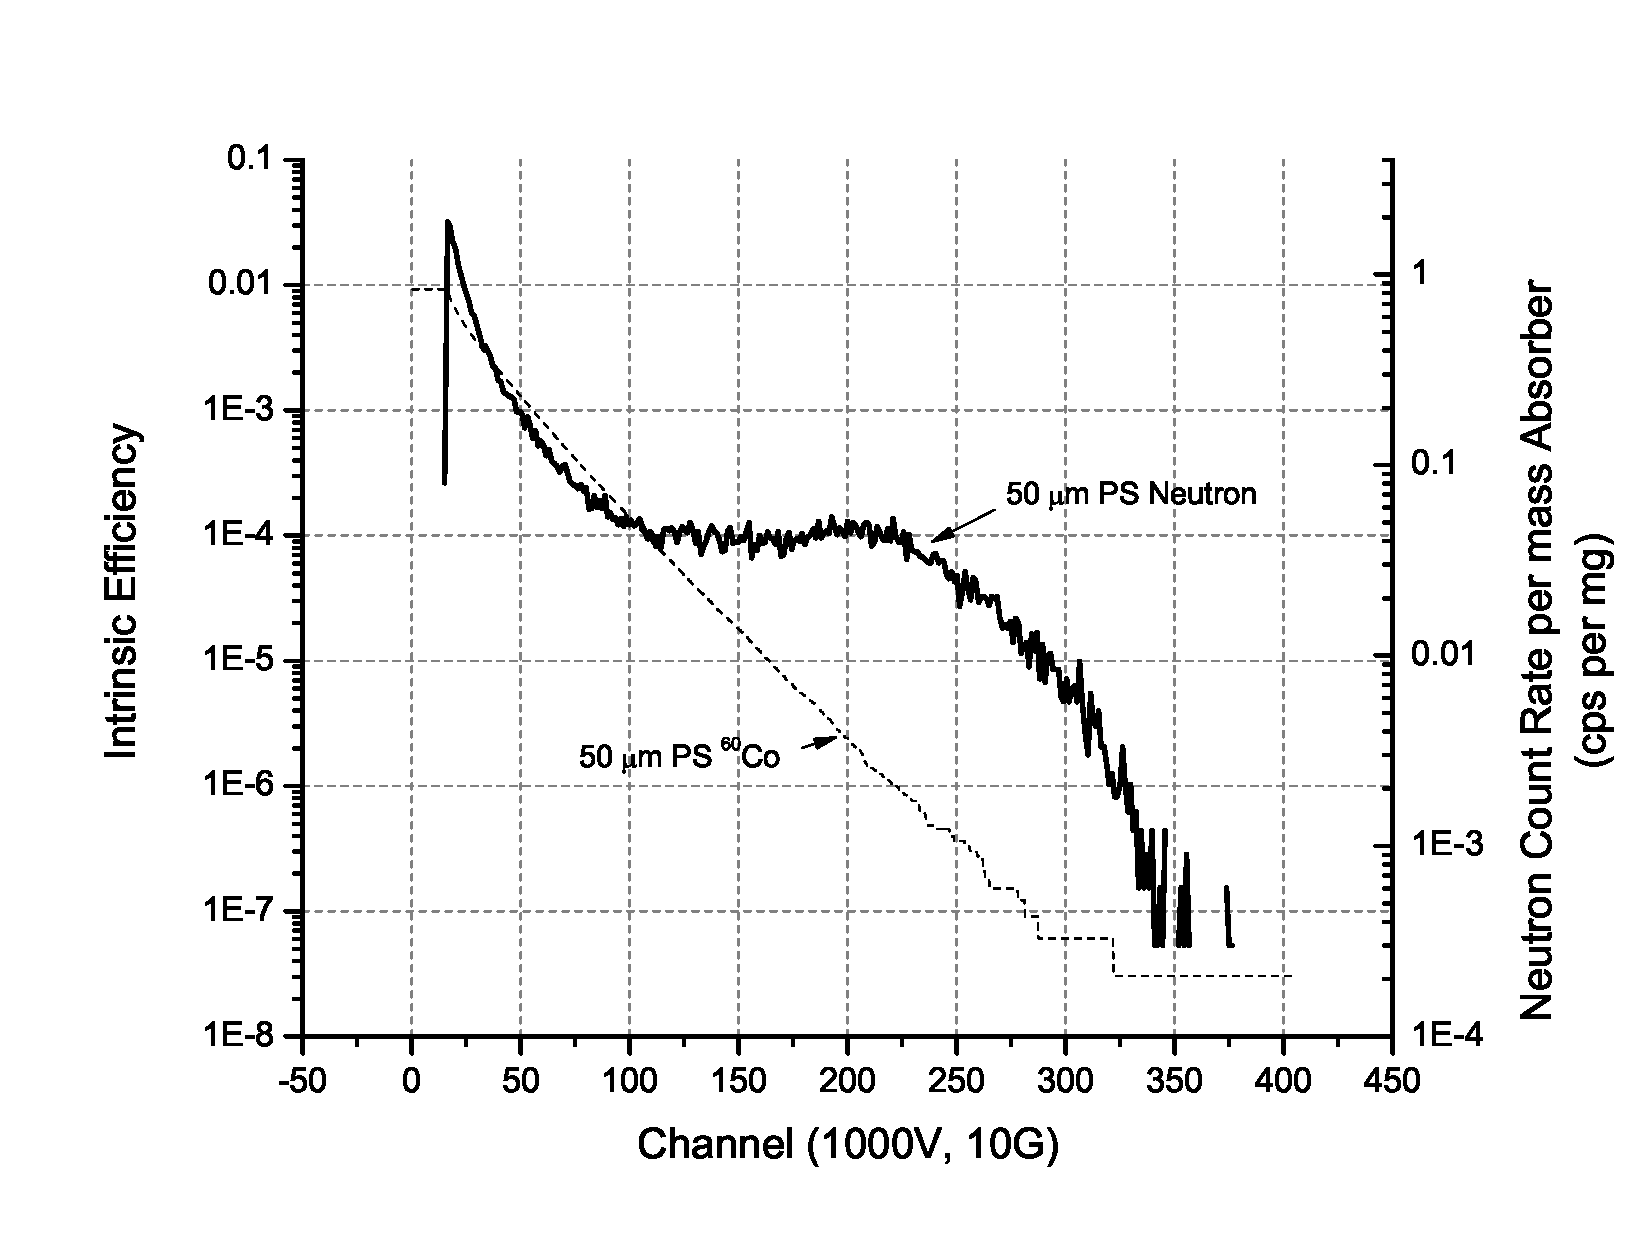
\includegraphics[width=\textwidth]{SC_PS_IntEff_CR}
  \caption[Cast Polystyrene Performance]{Performance of an \SI{50}{\um}, 10\% \iso[6]{LiF} PS Film (24 Jan 2012 Sample).}
  \label{fig:PSPreformance}
\end{figure}
\begin{figure}
  \centering
  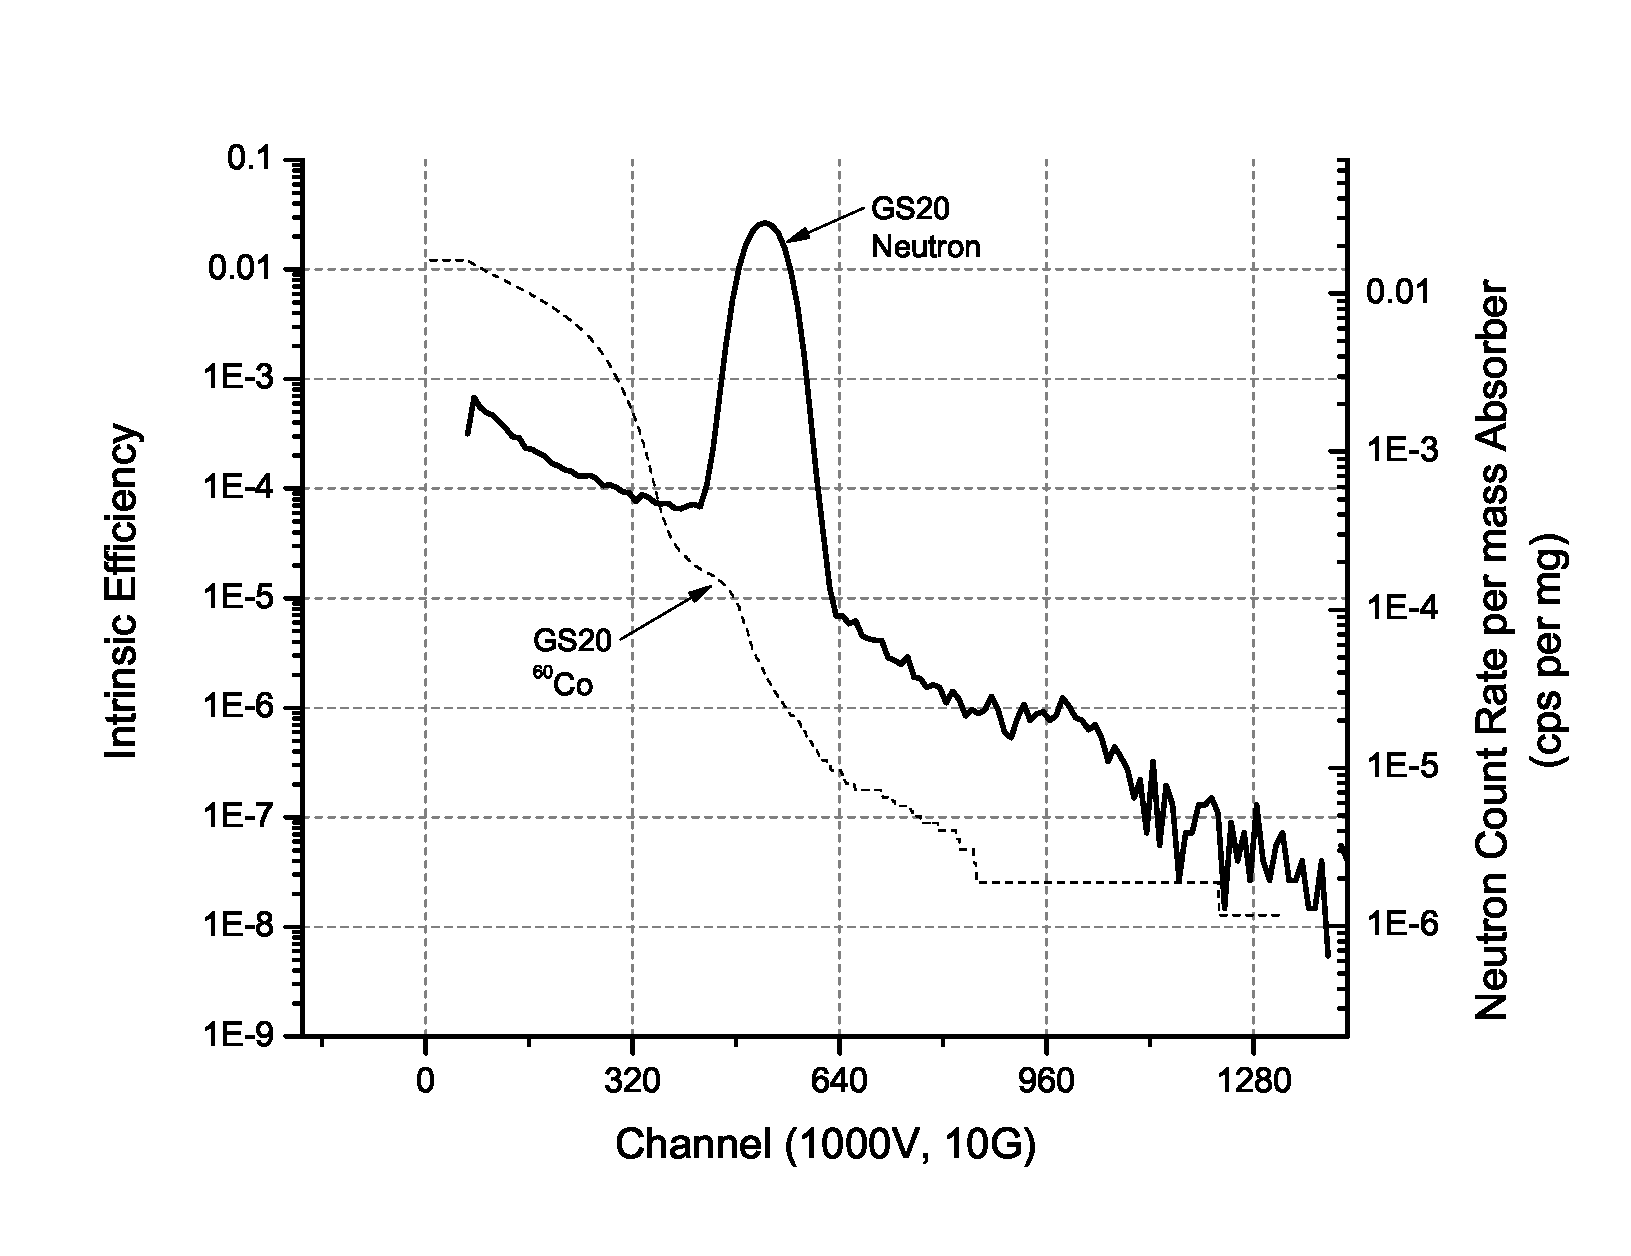
\includegraphics[width=\textwidth]{SC_GS20_IntEff_CR}
  \caption[GS20 Performance]{Performance of \SI{2}{\mm} GS20.  It should be noted that there is significant self shielding in GS20, and that due to the gamma sensitivity catching the tail of the neutron peak the count rate above the gamma pulse height discriminator has the most variation of the samples measured.}
  \label{fig:GS20Preformance}
\end{figure}
\begin{figure}
  \centering
  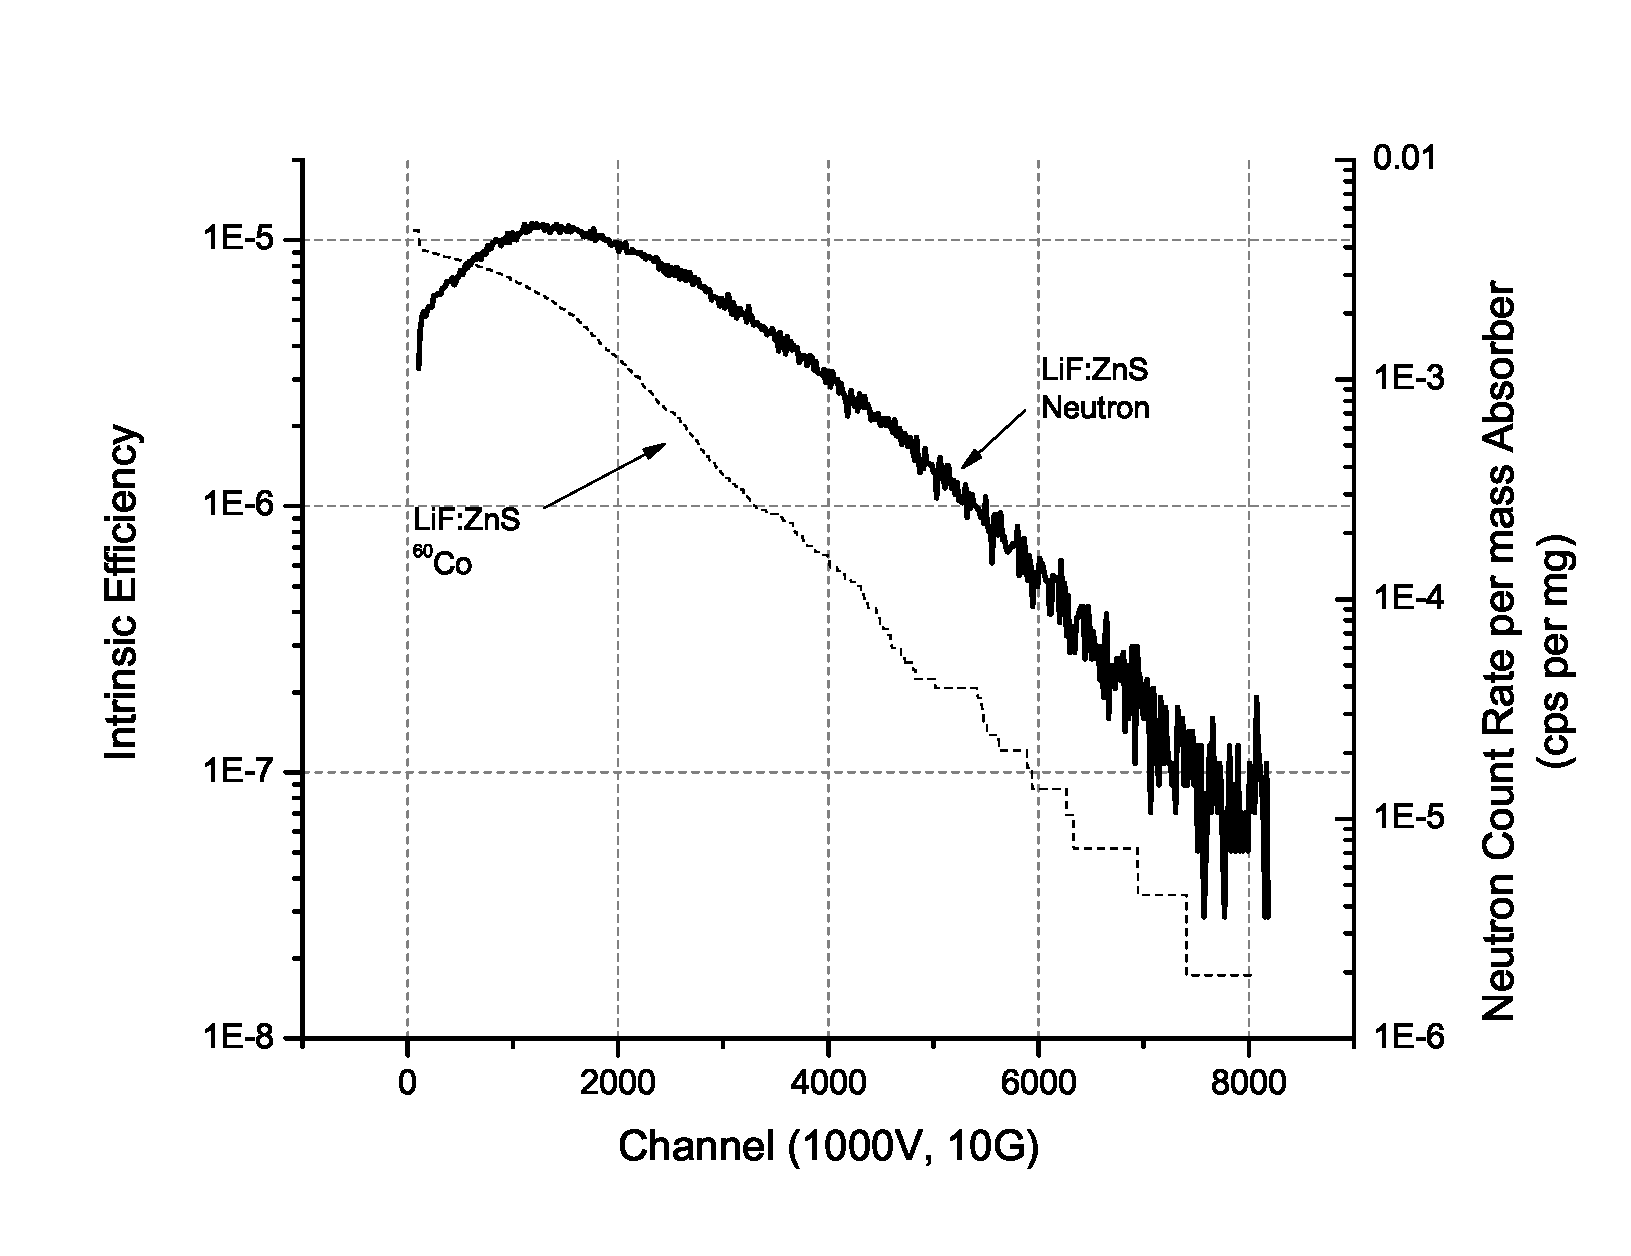
\includegraphics[width=\textwidth]{SC_EJ426_IntEff_CR}
  \caption[EJ 426 Performance]{Performance of EJ-426 HD2 (LiF:ZnS(Ag)) sheet.  This is the brightest scintillator tested, with the lowest gamma sensitivity.}
  \label{fig:EJ254Perf}
\end{figure}
\begin{figure}
  \centering
  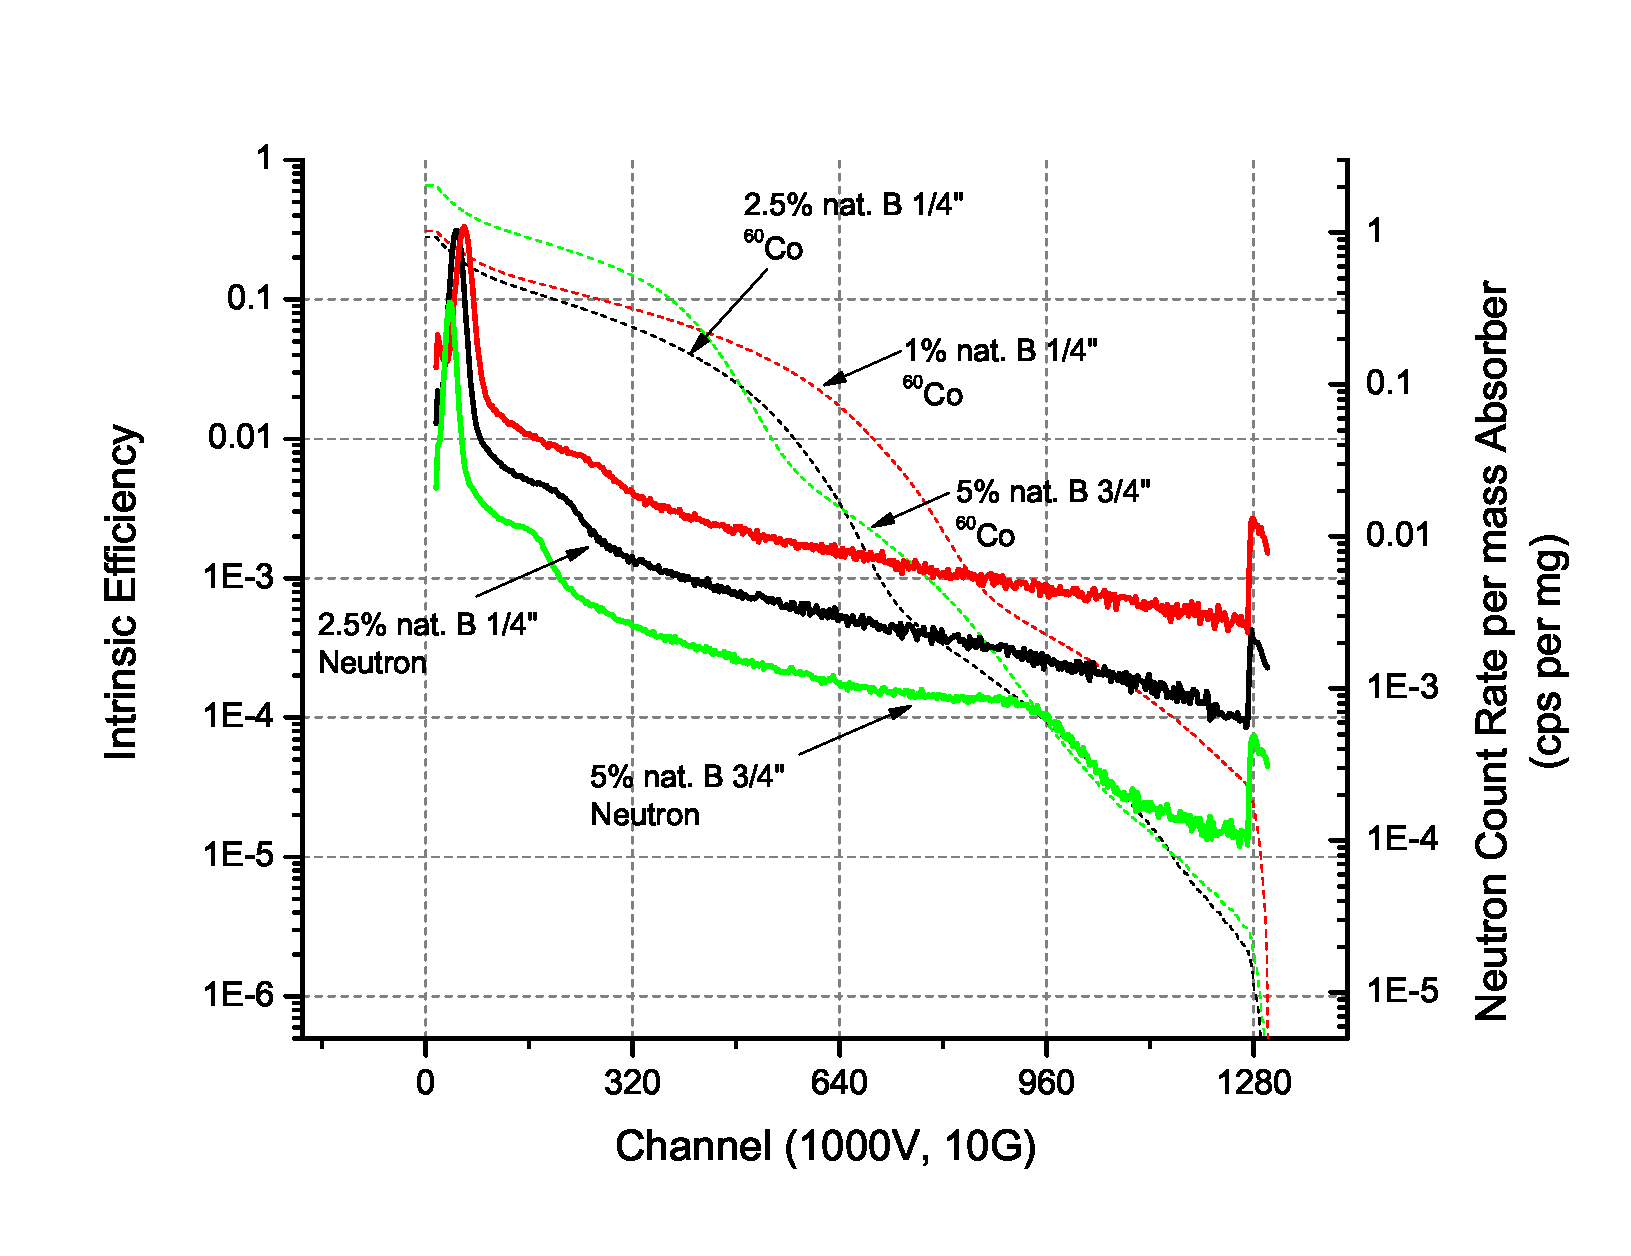
\includegraphics[width=\textwidth]{SC_EJ254_IntEff_CR}
  \caption[EJ 254 Performance]{Performance of EJ-254}
  \label{fig:EJ254Preformance}
\end{figure}
It is apparent that the EJ-254 is not a suitable candidate for replacement detector material in an RPM using a pulse height discriminator.
The reasons for this are twofold: 1) the detector is very thick which increases the probability of a gamma interaction as well as the probability that the interaction will deposit a majority of its energy and 2) \iso[10]{B} has a much lower Q-value (\SI{2.78}{\MeV} compared to \SI{4.78}{\MeV}) and a large pulse height deficit.
However, the material is optically transparent and due to \iso[10]{B}'s large thermal perhaps a thin sheet of EJ-254 might make a suitable detector material.

    %%%%%%%%%%%%%%%%%%%%%%%%%%%%%%%%%%%%%%%%%%%%%%%%%%%%%%%%%%%%%%%%%%%%%%%%%%%
    % A VITA IS REQUIRED
    %%%%%%%%%%%%%%%%%%%%%%%%%%%%%%%%%%%%%%%%%%%%%%%%%%%%%%%%%%%%%%%%%%%%%%%%%%%
    \addToTOC{Vita}
    \chapter*{Vita} \label{ch:vita}
Matthew J. Urffer was born January, 29, 1988 on a small turkey farm on Urffer Road in Coopersburg, Pa.
He got his B.S. in physics from Carnegie Mellon University in Pittsburgh, PA. 
Upon graduation Matthew enrolled at the University of Tennessee, Knoxville where he received his Masters in Nuclear Engineering in December, 2012 and his doctorate in nuclear engineering in December, 2013.

\end{document}
